\documentclass[
]{article}
\usepackage{amsmath,amssymb}
\usepackage{lmodern}
\usepackage{iftex}
\usepackage{graphicx}
\usepackage{float}
\usepackage{hyperref}
\ifPDFTeX
\usepackage[T1]{fontenc}
\usepackage[utf8]{inputenc}
\usepackage{textcomp} % provide euro and other symbols
\else % if luatex or xetex
\usepackage{unicode-math}
\defaultfontfeatures{Scale=MatchLowercase}
\defaultfontfeatures[\rmfamily]{Ligatures=TeX,Scale=1}
\fi
% Use upquote if available, for straight quotes in verbatim environments
\IfFileExists{upquote.sty}{\usepackage{upquote}}{}
\IfFileExists{microtype.sty}{% use microtype if available
    \usepackage[]{microtype}
    \UseMicrotypeSet[protrusion]{basicmath} % disable protrusion for tt fonts
}{}
\makeatletter
\@ifundefined{KOMAClassName}{% if non-KOMA class
    \IfFileExists{parskip.sty}{%
        \usepackage{parskip}
    }{% else
        \setlength{\parindent}{0pt}
        \setlength{\parskip}{6pt plus 2pt minus 1pt}}
}{% if KOMA class
    \KOMAoptions{parskip=half}}
\makeatother
\usepackage{xcolor}
\usepackage{longtable,booktabs,array}
\usepackage{calc} % for calculating minipage widths
% Correct order of tables after \paragraph or \subparagraph
\usepackage{etoolbox}
\makeatletter
\patchcmd\longtable{\par}{\if@noskipsec\mbox{}\fi\par}{}{}
\makeatother
% Allow footnotes in longtable head/foot
\IfFileExists{footnotehyper.sty}{\usepackage{footnotehyper}}{\usepackage{footnote}}
\makesavenoteenv{longtable}
\usepackage{graphicx}
\makeatletter
\def\maxwidth{\ifdim\Gin@nat@width>\linewidth\linewidth\else\Gin@nat@width\fi}
\def\maxheight{\ifdim\Gin@nat@height>\textheight\textheight\else\Gin@nat@height\fi}
\makeatother
% Scale images if necessary, so that they will not overflow the page
% margins by default, and it is still possible to overwrite the defaults
% using explicit options in \includegraphics[width, height, ...]{}
\setkeys{Gin}{width=\maxwidth,height=\maxheight,keepaspectratio}
% Set default figure placement to htbp
\makeatletter
\def\fps@figure{htbp}
\makeatother
\setlength{\emergencystretch}{3em} % prevent overfull lines
\providecommand{\tightlist}{%
    \setlength{\itemsep}{0pt}\setlength{\parskip}{0pt}}
\setcounter{secnumdepth}{-\maxdimen} % remove section numbering
\ifLuaTeX
\usepackage{selnolig}  % disable illegal ligatures
\fi
\IfFileExists{bookmark.sty}{\usepackage{bookmark}}{\usepackage{hyperref}}
\IfFileExists{xurl.sty}{\usepackage{xurl}}{} % add URL line breaks if available
\urlstyle{same} % disable monospaced font for URLs
\hypersetup{
    hidelinks,
    pdfcreator={LaTeX via pandoc}}

\author{}
\date{}

\begin{document}
    \thispagestyle{empty}
    \textbf{Šablona závěrečné práce\\
    studenta Unicorn Vysoká škola}

    \emph{Tato první stránka šablony není součástí bakalářské práce.}

    \emph{Tato šablona slouží jako vzorová šablona závěrečných prací
    studentům Unicorn Vysoké školy. Závěrečná práce musí obsahovat všechny
    náležitosti uvedené v této šabloně.}

    \emph{Nesplnění této podmínky může být považováno za důvod pro
    nepřipuštění závěrečné práce k obhajobě (nebo případně k vrácení práce
    od obhajoby k přepracování).}

    \emph{Další informace a pokyny k vypracování závěrečná práce naleznete
    na webových stránkách. Vše potřebné se také dozvíte v~rámci předmětu
    Bakalářský seminář.}

    \emph{Při zpracování této šablony bylo použito písmo Cambria, 11pt. pro
    text a písmo Calibri pro nadpisy.}

    \newpage
    \pagebreak
    \begin{quote}
        \thispagestyle{empty}
        \emph{Vzor: \textbf{PEVNÁ DESKA} závěrečné práce \textbf{není součástí
        elektronické verze}}
        \textbf{UNICORN VYSOKÁ ŠKOLA S.R.O.}

        \hspace{0pt}
        \vfill
        BAKALÁŘSKÁ/DIPLOMOVÁ PRÁCE (vyberte jednu možnost)
        \vfill
        \hspace{0pt}

        \textbf{Rok Jméno a PŘÍJMENÍ autora}
        \emph{\textbf{(Jan NOVÁK)}}
        \pagebreak
    \end{quote}

    \newpage
    \begin{quote}
        \thispagestyle{empty}
        \emph{Vzor: \textbf{TITULNÍ STRANA} závěrečné práce}

        \textbf{UNICORN VYSOKÁ ŠKOLA S.R.O.}

        \textbf{Softwarové inženýrství a big data}

        % \includegraphics[width=3.27778in,height=3.90671in]{vertopal_c6b44323f8f4439b87d257a2a20a5c78/media/image4.png}

        \textbf{DIPLOMOVÁ PRÁCE (vyberte jednu možnost)}

        \textbf{Název práce (přesně podle zadání)}

        \textbf{Autor BP:} Jméno a příjmení autora/autorky (Jan Novák)

        \textbf{Vedoucí BP:} Jméno a příjmení vedoucí/vedoucího práce i s tituly
        (prof. Ing. Jan Čadil, Ph.D.)

        \newpage
        \thispagestyle{empty}
        \emph{Vzor: \textbf{ZADÁNÍ ZÁVĚREČNÉ PRÁCE} -- originál, kopie
        originálu, naskenovaná podoba -- dle jednotlivých forem (originál, 2 x
        kopie, elektronická verze)}

        \newpage
        \thispagestyle{empty}
        \emph{Vzor: \textbf{ČESTNÉ PROHLÁŠENÍ} -- prohlášení o samostatném
        vypracování závěrečné práce, datum a vlastnoruční podpis (v každém
        výtisku práce)}

        \textbf{Čestné prohlášení}

        Prohlašuji, že jsem svou bakalářskou práci na téma
        ....................... vypracoval/a samostatně pod vedením vedoucího
        bakalářské práce a s použitím výhradně odborné literatury a dalších
        informačních zdrojů, které jsou v práci všechny citovány a jsou také
        uvedeny v seznamu použitých zdrojů.

        Jako autor/ka této bakalářské práce dále prohlašuji, že v souvislosti s
        jejím vytvořením jsem neporušil/a autorská práva třetích osob a jsem si
        plně vědom/a následků porušení ustanovení § 11 a následujících
        autorského zákona č. 121/2000 Sb. Prohlašuji, že nástroje umělé inteligence byly využity pouze po podpůrné činnosti a v souladu s principem akademické etiky.

        Dále prohlašuji, že odevzdaná tištěná verze bakalářské práce je shodná
        s~verzí, která byla odevzdána elektronicky.

        V\ldots\ldots\ldots\ldots\ldots\ldots\ldots\ldots. dne
        \ldots\ldots\ldots..
        \ldots\ldots.\ldots\ldots\ldots\ldots\ldots\ldots\ldots\ldots\ldots\ldots\ldots{}

        (Jan Novák)

        \newpage
        \thispagestyle{empty}
        \emph{Vzor: \textbf{PODĚKOVÁNÍ} vedoucímu BP, konzultantům, odborníků,
            spolupracovníkům za poskytnuté rady a podkladové materiály apod.) --
            \textbf{není povinné}}

        \textbf{Poděkování}

        Např: Děkuji vedoucímu bakalářské práce Jméno Příjmení (i s tituly) za
        účinnou metodickou, pedagogickou a odbornou pomoc a další cenné rady při
        zpracování mé bakalářské práce\ldots{}

        \newpage
        \emph{Vzor: \textbf{PRVNÍ ČÍSLOVANÁ STRANA} -- číslice na první
        číslované straně se určí podle počtu předchozích stran, počínaje Titulní
        stranou, tzn. že pokud jsou řazené všechny dané strany -- Titulní
        strana, Zadání (2 strany), Čestné prohlášení a Poděkování -- je první
        číslovaná strana stranou 6.}
    \end{quote}

    \begin{quote}
        \textbf{Název práce v českém/slovenském jazyce Název práce v anglickém
        jazyce}
    \end{quote}

    \emph{Vzor: ABSTRAKT A KLÍČOVÁ SLOVA}

    \begin{quote}
        \textbf{Abstrakt}

        Abstrakt česky. Abstrakt krátce a výstižně charakterizuje obsah
        závěrečné práce. Zpravidla obsahuje informace o stanovených cílech,
        použitých metodách, postupu řešení a výsledcích výzkumu. Může obsahovat
        krátkou informaci o použitých zdrojích. Délka abstraktu je zpravidla
        100--500 slov.

        Klíčová slova: klíčová slova práce, minimálně 5, maximálně 10

        \textbf{Abstract}

        Zde umístěte překlad abstraktu do anglického jazyka. Česky a anglicky
        psané abstrakty musí být totožné. Student/ka zodpovídá za jazykovou
        správnost anglického překladu. V případě, že se anglická a česká verze
        nevejdou na jednu stránku, umístěte celý překlad na samostatnou stránku.

        Keywords: klíčová slova v~anglickém jazyce

        \newpage
        \emph{Vzor: \textbf{OBSAH} -- hierarchické uspořádání číslovaných názvů
        kapitol a podkapitol, včetně všech příloh, spolu s čísly jejich stran.
        Dále se uvádí Seznam obrázků/tabulek/grafů. Pozn.: počet a názvy kapitol
        samozřejmě odpovídají charakteru konkrétní práce.}

        \textbf{Obsah}
    \end{quote}
%
%    \hypertarget{section}{%
%
%
%        \section{}\label{section}}
%
%    \protect\hyperlink{uxfavod}{Úvod \protect\hyperlink{uxfavod}{9}}
%
%    \protect\hyperlink{teoretickuxe1-ux10duxe1st-nenuxed-nuxe1zev-kapitoly}{1
%    Overview of Heuristic and Meta-heuristic Optimization Algorithms
%    \protect\hyperlink{teoretickuxe1-ux10duxe1st-nenuxed-nuxe1zev-kapitoly}{10}}
%
%    \protect\hyperlink{nadpis-uxfarovnux11b-2}{1.1 Nadpis úrovně 2
%    \protect\hyperlink{nadpis-uxfarovnux11b-2}{10}}
%
%    \protect\hyperlink{nadpis-uxfarovnux11b-3}{1.1.1 Nadpis úrovně 3
%    \protect\hyperlink{nadpis-uxfarovnux11b-3}{10}}
%
%    \protect\hyperlink{nadpis-uxfarovnux11b-3-1}{1.1.2 Nadpis úrovně 3
%    \protect\hyperlink{nadpis-uxfarovnux11b-3-1}{10}}
%
%    \protect\hyperlink{nadpis-uxfarovnux11b-2-1}{1.2 Nadpis úrovně 2
%    \protect\hyperlink{nadpis-uxfarovnux11b-2-1}{10}}
%
%    \protect\hyperlink{nadpis-uxfarovnux11b-3-2}{1.2.1 Nadpis úrovně 3
%    \protect\hyperlink{nadpis-uxfarovnux11b-3-2}{10}}
%
%    \protect\hyperlink{nadpis-uxfarovnux11b-3-3}{1.2.2 Nadpis úrovně 3
%    \protect\hyperlink{nadpis-uxfarovnux11b-3-3}{10}}
%
%    \protect\hyperlink{praktickuxe1-ux10duxe1stempirickuxe1-ux10duxe1stvlastnuxed-pruxe1ce-nenuxed-nuxe1zev-kapitoly}{2
%    Praktická část/Empirická část/Vlastní práce (není název kapitoly)
%        \protect\hyperlink{praktickuxe1-ux10duxe1stempirickuxe1-ux10duxe1stvlastnuxed-pruxe1ce-nenuxed-nuxe1zev-kapitoly}{11}}
%
%    \protect\hyperlink{nadpis-uxfarovnux11b-2-2}{2.1 Nadpis úrovně 2
%    \protect\hyperlink{nadpis-uxfarovnux11b-2-2}{11}}
%
%    \protect\hyperlink{zuxe1vux11br}{Závěr
%    \protect\hyperlink{zuxe1vux11br}{13}}

%    \protect\hyperlink{seznam-pouux17eituxfdch-zdrojux16f}{Seznam použitých
%    zdrojů \protect\hyperlink{seznam-pouux17eituxfdch-zdrojux16f}{14}}
%
%    \protect\hyperlink{seznam-obruxe1zkux16f-existujuxed-li}{Seznam obrázků
%        (existují-li)
%        \protect\hyperlink{seznam-obruxe1zkux16f-existujuxed-li}{15}}
%
%    \protect\hyperlink{seznam-grafux16f-existujuxed-li}{Seznam grafů
%        (existují-li) \protect\hyperlink{seznam-grafux16f-existujuxed-li}{17}}
%
%    \protect\hyperlink{seznam-pux159uxedloh-existujuxed-li}{Seznam příloh
%        (existují-li)
%        \protect\hyperlink{seznam-pux159uxedloh-existujuxed-li}{18}}
%
%    \protect\hyperlink{pux159uxedloha-a-nuxe1zev-pux159uxedlohy}{Příloha A
%    -- Název přílohy
%    \protect\hyperlink{pux159uxedloha-a-nuxe1zev-pux159uxedlohy}{19}}
%
%    \protect\hyperlink{pux159uxedloha-b-nuxe1zev-pux159uxedlohy}{Příloha B
%    -- Název přílohy
%    \protect\hyperlink{pux159uxedloha-b-nuxe1zev-pux159uxedlohy}{20}}
    \tableofcontents

    \newpage


    \section{Introduction}\label{sec:uxfavod}

    \subsection{Hypotheses}\label{subsec:hypotheses}
    \begin{enumerate}
        \item \textbf{Hypothesis 1:} The implementation of heuristic optimization algorithms, such as genetic algorithms, simulated annealing, and tabu search, will significantly improve the efficiency of route planning in logistics, leading to reduced delivery times and operational costs compared to traditional methods.
        \item \textbf{Hypothesis 2:} The integration of multiple heuristic algorithms will create a robust and flexible optimization framework capable of adapting to dynamic changes and uncertainties in logistics operations, thereby enhancing overall performance and reliability.
        \item \textbf{Hypothesis 3:} Using simulation tools to test and validate heuristic optimization algorithms will demonstrate their practical feasibility and effectiveness in real-world logistics scenarios, highlighting both their strengths and potential areas for improvement.
    \end{enumerate}

    \subsection{Research Questions}\label{subsec:research_questions}
    \begin{itemize}
        \item What are the main advantages and disadvantages of individual heuristic optimization algorithms compared to traditional methods in logistics route planning?
        \item How does the integration of multiple heuristic algorithms affect the system's ability to handle dynamic changes and uncertainties in logistics operations?
        \item To what extent can simulation tools contribute to the validation and improvement of heuristic optimization algorithms in real-world logistics scenarios?
        \item What specific scenarios and parameters should be considered when designing simulation experiments to test the performance of heuristic algorithms in logistics?
    \end{itemize}


    \newpage

    \hypertarget{vehicle-routing-problem}{%


        \section{Vehicle Routing Problem (VRP)}\label{vehicle-routing-problem}}


    \hypertarget{introduction-to-the-vehicle-routing-problem}{%

        \subsection{Introduction to the Vehicle Routing Problem}\label{introduction-to-the-vehicle-routing-problem}}

    The Vehicle Routing Problem (VRP) occupies a central place in operational research and logistics due to its direct applicability to optimizing the distribution of goods and services. First formulated by Dantzig and Ramser in 1959, the VRP has evolved significantly, encompassing various complex forms tailored to different industrial needs and constraints.

    \subsubsection{Historical Background and Significance}\label{subsubsec:historical-background-and-significance}
    The VRP, initially introduced as the "Truck Dispatching Problem" by Dantzig and Ramser (1959), seeks to determine the most efficient routes for a fleet of delivery vehicles operating from a central depot. This problem is foundational in the field of combinatorial optimization and remains pivotal in supply chain management and logistics.

    \subsubsection{Problem Definition}\label{subsubsec:problem_definition}


    At its core, the Vehicle Routing Problem (VRP) involves designing optimal routes for a fleet of vehicles that must deliver goods or services to a set of customers and return to the depot, minimizing total travel costs while satisfying various constraints. This classic problem not only focuses on reducing operational expenses but also on improving service efficiency and customer satisfaction.

    \paragraph{Objective:}
    The primary objective of the VRP is to determine a set of routes that minimizes the total cost of transportation. Costs typically include distance traveled, time spent, fuel consumption, and sometimes additional factors such as toll charges or vehicle maintenance. The total cost must be minimized while ensuring that all customer demands are met and all operational constraints are adhered to.

    \paragraph{Constraints:}
    Several constraints must be considered in the VRP:
    \begin{itemize}
        \item \textbf{Capacity Constraints}: Each vehicle has a maximum carrying capacity that must not be exceeded by the sum of the demands of the customers it serves. This ensures that the vehicle can physically carry the load assigned to it without overloading.
        \item \textbf{Route Length Constraints}: Often, there is a maximum allowable route length or time duration for each vehicle's tour, which might be dictated by legal driving hours, fuel limitations, or service level agreements.
        \item \textbf{Customer Constraints}: Each customer must be visited exactly once by one vehicle. In cases involving time windows, each customer must be serviced within a specific time frame.
        \item \textbf{Depot Constraints}: All routes must start and end at the depot, ensuring the cyclic nature of vehicle tours.
    \end{itemize}

% \paragraph{Formulation:}
% Mathematically, the VRP can be represented using a graph \( G = (V, E) \), where \( V \) is the set of vertices (nodes) including the depot and customers, and \( E \) is the set of edges (arcs) representing possible routes between vertices. The problem is often formulated as an integer programming model where decision variables indicate whether a route between two vertices is included in the solution. The objective function minimizes the total cost associated with the selected routes, subject to the aforementioned constraints.

    \paragraph{Formulation:}
    Mathematically, the VRP can be represented using a graph \( G = (V, E) \), where \( V \) is the set of vertices (nodes) including the depot and customers, and \( E \) is the set of edges (arcs) representing possible routes between vertices. Each edge \( (i, j) \in E \) is associated with a cost \( c_{ij} \), which typically represents the distance or travel time between vertices \( i \) and \( j \).

    The problem is often formulated as an integer programming model where decision variables indicate whether a route between two vertices is included in the solution. Let \( x_{ij} \) be a binary decision variable that equals 1 if edge \( (i, j) \) is included in the route and 0 otherwise. The objective function is to minimize the total cost associated with the selected routes, subject to various constraints.

    \begin{equation}
        \min \sum_{(i,j) \in E} c_{ij} x_{ij}
    \end{equation}

    The objective function aims to minimize the total travel cost. The formulation includes several constraints to ensure the solution is feasible:

    \paragraph{Degree Constraints:}
    Each customer must be visited exactly once, which can be represented as:
    \begin{equation}
        \sum_{j \in V, j \neq i} x_{ij} = 1 \quad \forall i \in V \setminus \{0\}
    \end{equation}
    \begin{equation}
        \sum_{i \in V, i \neq j} x_{ij} = 1 \quad \forall j \in V \setminus \{0\}
    \end{equation}

    These constraints ensure that each customer node \( i \) has exactly one incoming and one outgoing edge, forming a valid route.

    \paragraph{Capacity Constraints:}
    Each vehicle has a limited capacity \( Q \). Let \( q_i \) be the demand at customer \( i \). The total demand serviced by a vehicle on its route must not exceed its capacity. This can be formulated using flow variables \( u_i \) representing the load of the vehicle after visiting customer \( i \):

    \begin{equation}
        u_i - u_j + Q x_{ij} \leq Q - q_j \quad \forall (i, j) \in E, i \neq j, i \neq 0
    \end{equation}

    \begin{equation}
        q_i \leq u_i \leq Q \quad \forall i \in V \setminus \{0\}
    \end{equation}

    Here, \( u_i \) is set to 0 at the depot.

    \paragraph{Subtour Elimination Constraints:}
    To prevent the formation of subtours (cycles that do not include the depot), we use subtour elimination constraints. For example, in the Miller-Tucker-Zemlin (MTZ) formulation:

    \begin{equation}
        u_i - u_j + Q x_{ij} \leq Q - q_i \quad \forall (i, j) \in E, i \neq j, i \neq 0
    \end{equation}

    \begin{equation}
        q_i \leq u_i \leq Q \quad \forall i \in V \setminus \{0\}
    \end{equation}

    \paragraph{Depot Constraints:}
    All routes must start and end at the depot:

    \begin{equation}
        \sum_{j \in V \setminus \{0\}} x_{0j} = m
    \end{equation}
    \begin{equation}
        \sum_{i \in V \setminus \{0\}} x_{i0} = m
    \end{equation}

    where \( m \) is the number of vehicles available.

    \paragraph{Flow Conservation Constraints:}
    These constraints ensure the flow conservation at each node, meaning the number of vehicles entering a customer node must equal the number leaving it:

    \begin{equation}
        \sum_{j \in V \setminus \{i\}} x_{ij} = \sum_{j \in V \setminus \{i\}} x_{ji} \quad \forall i \in V \setminus \{0\}
    \end{equation}

    This comprehensive formulation ensures that all aspects of the VRP are covered, including minimizing travel costs, adhering to vehicle capacities, servicing all customers exactly once, starting and ending routes at the depot, and preventing subtours. The problem is complex due to the combination of these constraints, which necessitates advanced optimization techniques for finding feasible and near-optimal solutions in practical applications.

    \paragraph{Applications:}
    The VRP is highly relevant across various industries, including logistics, supply chain management, waste collection, and public transportation. Effective solutions to VRP can lead to significant cost savings, improved service levels, and enhanced operational efficiency.

    \paragraph{Research and Development:}
    The study of VRP has led to significant advancements in optimization theory and practice. Researchers have developed a wide range of solution methodologies, from classical operations research techniques to modern metaheuristics and machine learning approaches. Continuous improvement in computational power and algorithmic strategies promises ongoing advancements in solving VRP more efficiently and effectively.

    This comprehensive overview of the VRP problem definition provides a solid foundation for understanding its complexities and importance, setting the stage for detailed exploration of its variants and solution methods in the subsequent sections.

    \subsection{Complexity and Relevance}\label{subsec:complexity-and-relevance}
    The VRP is known to be NP-hard, implying that no efficient algorithm can solve all instances optimally in polynomial time. This complexity necessitates sophisticated solution approaches, both exact and heuristic, to find feasible and near-optimal solutions efficiently.

    \subsection{Variants and Extensions}\label{subsec:variants-and-extensions}
    There are numerous variants of the VRP, each introducing additional layers of complexity to address real-world logistics challenges. These variants reflect the diverse operational requirements and constraints encountered in practical applications. Key variants include:


    \begin{itemize}
        \item \textbf{Capacitated VRP (CVRP)}:
        The CVRP is the most widely studied variant of the VRP, focusing on the distribution of goods from a single depot to multiple customers using a fleet of vehicles with fixed capacities. Each vehicle must deliver goods without exceeding its capacity, and the objective is to minimize the total cost, typically the travel distance or time. This variant is fundamental in understanding more complex VRP forms and is used extensively in both academic research and practical applications.

        \item \textbf{VRP with Time Windows (VRPTW)}:
        The VRPTW adds the complexity of time constraints to the basic VRP. Each customer must be serviced within a specified time window, adding another layer of complexity to the routing problem. This variant is crucial for industries where delivery times are critical, such as perishable goods distribution and courier services. The goal is to minimize the total travel cost while ensuring that all deliveries or pickups occur within their designated time frames. Time windows make the problem significantly harder to solve, and specialized algorithms, often involving sophisticated scheduling techniques, are required.

        \item \textbf{Dynamic VRP (DVRP)}:
        In the DVRP, the problem parameters, such as customer requests or traffic conditions, change dynamically over time. This variant reflects real-world situations where information is not static and decisions must be adapted in real-time. For example, new customer orders might arrive throughout the day, or unexpected traffic jams might alter the planned routes. Solving the DVRP requires algorithms that can efficiently update solutions in response to new information, often leveraging real-time data and adaptive heuristics.

        \item \textbf{Stochastic VRP (SVRP)}:
        The SVRP deals with uncertainty in problem data, such as variable customer demand or unpredictable travel times. This variant introduces probabilistic elements into the routing problem, requiring solutions that are robust to variability and can handle unexpected changes efficiently. Approaches to solving the SVRP often involve stochastic modeling and optimization techniques that consider multiple scenarios or employ probabilistic constraints.

        \item \textbf{Green VRP}:
        The Green VRP focuses on minimizing environmental impacts, such as fuel consumption and CO2 emissions, in addition to traditional cost metrics. This variant is increasingly important due to growing environmental regulations and the need for sustainable logistics practices. Green VRP models incorporate factors like vehicle emissions, fuel efficiency, and alternative energy sources into the optimization process. Methods to address Green VRP include eco-friendly routing algorithms and multi-objective optimization techniques.

    \end{itemize}

    \paragraph{Methodological Approaches}
    To tackle the VRP, both exact and heuristic methods have been developed, each with its strengths and weaknesses depending on the problem size and specific requirements.

    \paragraph{Exact Methods:}
    Exact methods guarantee finding an optimal solution by exhaustively exploring the solution space. These methods include:

    \begin{itemize}
        \item \textbf{Integer Programming (IP)}: IP formulations, such as the one presented earlier, model the VRP using binary variables and linear constraints. Solving IPs can yield optimal solutions, but the computational effort increases exponentially with problem size. Advanced techniques like Branch-and-Cut algorithms are often employed to handle larger instances by incorporating cutting planes to reduce the feasible region iteratively \cite{Toth2002}.
        \item \textbf{Branch and Bound (B\&B)}: This method systematically explores branches of a tree representing subsets of the solution space. By calculating bounds on the best possible solution within each subset, B\&B can prune large portions of the tree, thus reducing the number of solutions that need to be examined \cite{Laporte1992}.
        \item \textbf{Dynamic Programming (DP)}: DP breaks down the VRP into simpler subproblems and solves them recursively. While highly effective for smaller instances, the state space grows exponentially with the number of customers, limiting its practicality for large-scale problems.
    \end{itemize}

    \hypertarget{heuristic-and-metaheuristic-methods}{%


        \section{Heuristic and Metaheuristic Methods}\label{itm:heuristic-and-metaheuristic-methods}}

    Heuristic and metaheuristic methods provide near-optimal solutions more efficiently, making them suitable for larger instances where exact methods are impractical. These methods do not guarantee optimality but are designed to produce good quality solutions within reasonable computational times.

    \begin{itemize}
        \item \textbf{Genetic Algorithms (GA):} Inspired by natural selection, GAs evolve a population of solutions using selection, crossover, and mutation to improve solution quality.
        \item \textbf{Simulated Annealing (SA):} A probabilistic technique that mimics the annealing process, allowing occasional worse solutions to escape local optima.
        \item \textbf{Tabu Search (TS):} Enhances local search by using a memory structure to avoid revisiting recently explored solutions, promoting thorough exploration.
        \item \textbf{Ant Colony Optimization (ACO):} Inspired by ant foraging behavior, ACO uses pheromone trails to guide the search for optimal paths.
        \item \textbf{Particle Swarm Optimization (PSO):} Simulates the social behavior of bird flocks or fish schools, where solutions (particles) move through the solution space based on their own and their neighbors' experiences.
    \end{itemize}

    A detailed discussion of these methods will be provided in a later chapter.

    \subsection{Conclusion and Outlook}\label{subsec:conclusion-and-outlook}
    As industries continue to seek improvements in operational efficiencies and cost reductions, the relevance of the VRP is expected to grow. Advances in computational power, data analytics, and artificial intelligence are opening new avenues for research and application, making the VRP a vibrant and ever-evolving field of study.

    This introduction provides a foundation for the comprehensive exploration of various aspects and complexities of the VRP, setting the stage for detailed discussions on its many variants and solving techniques in subsequent sections.
    \newpage


    \section{Introduction to the Capacitated Vehicle Routing Problem}\label{sec:intro_cvrp}

    The Capacitated Vehicle Routing Problem (CVRP) is a variant of the VRP that incorporates vehicle capacity constraints. This means each vehicle in the fleet has a maximum load it can carry, and the objective is to minimize the total cost of the routes while ensuring that the capacity constraints are not violated. The CVRP is critical in practical applications where load capacities are a significant factor, such as in logistics and supply chain management.

    \subsection{Importance and Applications}\label{subsec:importance-and-applications}

    CVRP is highly relevant in various industries due to its practical implications. For example, it is essential for urban delivery services, warehouse operations, and fleet management where adhering to vehicle capacities can significantly impact efficiency and cost-effectiveness.

    \subsection{Detailed Problem Definition}\label{subsec:detailed-problem-definition}

    At its core, the CVRP involves designing optimal routes for a fleet of vehicles that must deliver goods or services to a set of customers, ensuring that the load on each vehicle does not exceed its capacity. The primary objective is to minimize the total transportation cost, which typically includes distance traveled, time spent, and other operational expenses.

    \subsection{Key Constraints and Objectives}\label{subsec:key-constraints-and-objectives}

    \begin{itemize}
        \item \textbf{Capacity Constraints}: Each vehicle has a maximum carrying capacity that must not be exceeded by the sum of the demands of the customers it serves.
        \item \textbf{Route Length Constraints}: There is often a maximum allowable route length or time duration for each vehicle’s tour.
        \item \textbf{Customer Constraints}: Each customer must be visited exactly once by one vehicle.
        \item \textbf{Depot Constraints}: All routes must start and end at the depot.
    \end{itemize}

    \subsection{Mathematical Formulation}\label{subsec:mathematical-formulation}

    The Capacitated Vehicle Routing Problem (CVRP) can be mathematically formulated using a graph $G = (V, E)$, where $V$ is the set of vertices (nodes) including the depot and customers, and $E$ is the set of edges (arcs) representing possible routes between vertices. Each edge $(i, j) \in E$ is associated with a cost $c_{ij}$, representing the distance or travel time between vertices $i$ and $j$.

    In contrast to the general Vehicle Routing Problem (VRP), which focuses on minimizing the total cost of routes, the CVRP introduces an additional layer of complexity by incorporating vehicle capacity constraints. In CVRP, each vehicle $k$ has a maximum capacity $Q_k$, and each customer $i$ has a demand $d_i$ that must be satisfied without exceeding the vehicle's capacity.

    The objective of the CVRP is to minimize the total cost, given by:

    \begin{equation}
        \text{Minimize} \quad \sum_{k} \sum_{(i,j) \in E} c_{ij} x_{ij}^k
    \end{equation}

    subject to:

    1. \textbf{Capacity Constraints}: Ensure the total demand on each vehicle route does not exceed its capacity.
    \begin{equation}
        \sum_{i \in V} d_i x_{ij}^k \leq Q_k \quad \forall k
    \end{equation}

    2. \textbf{Customer Constraints}: Each customer is visited exactly once.
    \begin{equation}
        \sum_{k} \sum_{j \in V, j \neq i} x_{ij}^k = 1 \quad \forall i \in V \setminus \{0\}
    \end{equation}

    3. \textbf{Depot Constraints}: All routes start and end at the depot.
    \begin{equation}
        \sum_{j \in V \setminus \{0\}} x_{0j}^k = 1 \quad \forall k
    \end{equation}

    This formulation ensures that all aspects of the CVRP are covered, including minimizing travel costs, adhering to vehicle capacities, and ensuring each customer is visited exactly once, with all routes starting and ending at the depot.

    \subsection{Overview of Solution Approaches}\label{subsec:overview-of-solution-approaches}

    Many algorithms developed for the general VRP can also be applied to the CVRP, often with modifications to account for vehicle capacity constraints. These algorithms need to be adapted to ensure that solutions remain feasible concerning the capacity limits of the vehicles. For instance, the Clarke-Wright Savings Algorithm, originally designed for the VRP, can be adjusted to respect vehicle capacities by carefully merging routes. Similarly, Genetic Algorithms (GA) evolve solutions over generations and can be tailored to handle capacity constraints effectively through specific crossover and mutation operators. Ant Colony Optimization (ACO) mimics the foraging behavior of ants and can be adapted to consider both distance and load carried to ensure capacity constraints are met. Simulated Annealing (SA), a probabilistic technique, allows occasional worse solutions to escape local optima and can be modified to include capacity constraints in the cooling schedule.

    These methods illustrate how optimization techniques for the general VRP can be adapted to address the specific challenges of the CVRP. By focusing on these adapted methods, the thesis will explore how advanced optimization techniques can effectively handle the unique challenges posed by CVRP, aiming to find efficient and practical solutions for real-world logistics problems.

    \hypertarget{overview-of-heuristic-and-meta-heuristic-optimization-algorithms}{%


        \section{Overview of Heuristic and Meta-heuristic Optimization Algorithms}\label{overview-of-heuristic-and-meta-heuristic-optimization-algorithms}}



    In the fields of computational science and mathematical programming, a heuristic algorithm is a method used to find a good enough solution when it's not feasible to find the perfect solution. These algorithms focus on working quickly and efficiently rather than achieving flawless accuracy or the best possible result. They are especially valuable in situations where solving the problem completely and precisely would require too much computing power, or when the details of the problem are not fully known.

    Characteristics of Heuristic Algorithms:
    \begin{enumerate}
        \item \textbf{Approximation}: Heuristics do not guarantee that the solutions they provide will be optimal. Instead, they aim to deliver "good enough" solutions that are acceptable within practical constraints, such as limited processing time or resources.
        \item \textbf{Efficiency}: By not exhaustively searching every possible solution, heuristic algorithms can provide solutions much faster than their exact counterparts. This makes them especially valuable in dealing with large datasets or complex problem spaces where an exact approach would be computationally infeasible.
        \item \textbf{Adaptability}: Heuristic algorithms are often tailored to the specific characteristics of a problem, leveraging problem-specific insights and techniques to guide the search process towards more promising areas of the solution space.
    \end{enumerate}


    \hypertarget{common-types-of-heuristic-algorithms}{%

        \subsection{Common Types of Heuristic Algorithms}\label{itm:common-types-of-heuristic-algorithms}}

    \subsubsection{Greedy Algorithms}
    \label{subsubsec:greedy_algorithms}

    Greedy algorithms are a fundamental strategy in problem-solving, known for their focus on immediate benefits at each step. In every decision-making moment, a greedy algorithm selects the best immediate option, hoping that these short-term optimal choices will result in the best overall solution. While not always perfect, greedy algorithms are highly effective for many optimization problems due to their simplicity, speed, and often excellent results.

    The main feature of a greedy algorithm is the "greedy choice property," which means you can build an optimal solution step by step by making the best choice at each moment, without needing to rethink previous decisions. Once a decision is made, a greedy algorithm adheres to it, trusting that these decisions will lead to the best end result.

    Problems suited for greedy algorithms often exhibit an "optimal substructure," meaning that the best solution contains within it the best solutions to smaller problems. For instance, finding the shortest path in a network can be seen as finding the shortest paths to points along the way. This characteristic allows greedy algorithms to develop solutions progressively, focusing on the best choice at each step.

    \paragraph{Application Areas}

    Greedy algorithms are used across various fields due to their simplicity and efficiency. Some of the prominent application areas include:

    \begin{enumerate}
        \item \textbf{Scheduling:} Greedy algorithms are highly effective in scheduling tasks where immediate, optimal decisions can lead to efficient overall schedules. They are used to organize activities, sequence jobs, and manage time intervals. For instance, in job scheduling on machines, a greedy approach can be employed to minimize the total completion time by always assigning the next job to the machine that becomes available first. Additionally, in event scheduling, greedy algorithms help in assigning time slots to events to avoid conflicts, ensuring that no two events overlap. These algorithms are also used in task prioritization, where tasks are ordered based on deadlines or importance, allowing for efficient management of resources and time.

        \item \textbf{Graph Algorithms:} Greedy strategies are fundamental in graph theory, with several key applications such as finding the shortest paths in networks, constructing minimum spanning trees, and ensuring efficient traversal of graphs. These applications are critical in network routing, geographical mapping, and various optimization problems where optimal paths or connections are required.

        \item \textbf{Data Compression:} Greedy algorithms play a significant role in data compression techniques, optimizing storage and transmission efficiency. Huffman coding, a classic greedy algorithm, generates variable-length prefix codes based on the frequency of each data symbol. By assigning shorter codes to more frequent symbols and longer codes to less frequent symbols, Huffman coding minimizes the overall length of the encoded data. This approach is widely used in file compression formats such as ZIP and GZIP, as well as in multimedia codecs for compressing images, audio, and video. The efficiency of greedy algorithms in reducing data size without losing information makes them indispensable in modern data storage and communication.

        \item \textbf{Resource Allocation:} In scenarios where resources need to be allocated efficiently, greedy algorithms are employed to make optimal choices at each step. This includes tasks such as assigning tasks to workers, distributing goods among locations, and allocating bandwidth in communication networks. By continually selecting the most beneficial allocation at each step, these algorithms help in achieving near-optimal utilization of resources.

        \item \textbf{Financial Modeling:} Greedy algorithms are used in various financial models and decision-making processes. For example, in portfolio optimization, a greedy approach can be used to iteratively add assets to a portfolio based on their expected returns until the investment budget is exhausted. Similarly, in real-time bidding for online advertising, greedy algorithms help in making immediate bidding decisions to maximize the return on investment.

        \item \textbf{Route Planning:} In logistics and transportation, greedy algorithms are applied to route planning to minimize travel time or distance. This includes delivery route optimization, vehicle routing problems, and urban transit planning. By making locally optimal choices at each stage, these algorithms help in devising efficient routes that save time and fuel costs.

        \item \textbf{Machine Learning:} In the field of machine learning, greedy algorithms are used in feature selection and decision tree construction. By iteratively selecting the most relevant features or the best split at each node of a decision tree, these algorithms help in building efficient and accurate models for classification and regression tasks.

    \end{enumerate}

    \paragraph{Examples of Greedy Algorithms}

    \begin{enumerate}
        \item \textbf{Dijkstra’s Algorithm:} This algorithm finds the shortest path from a source node to all other nodes in a weighted graph. At each step, it selects the node with the smallest tentative distance from the source and updates the distances of its neighbors. The algorithm uses the following update rule:
        \[
            d(v) = \min \{ d(v), d(u) + w(u, v) \} \quad \text{for all } (u, v) \in E
        \]
        where \(d(v)\) is the tentative distance of vertex \(v\), and \(w(u, v)\) is the weight of the edge \((u, v)\).

        \item \textbf{Prim’s Algorithm:} Similar to Kruskal’s algorithm, Prim’s algorithm constructs a minimum spanning tree. It starts with an arbitrary node and repeatedly adds the nearest node that hasn’t been included in the tree yet. The inclusion criterion is:
        \[
            \text{Include } v \text{ such that } (u, v) \text{ is the smallest edge connecting } T \text{ to } V \setminus T
        \]
        where \(T\) is the set of nodes already included in the tree.

        \item \textbf{Kruskal’s Algorithm:} This algorithm constructs a minimum spanning tree for a connected weighted graph. It repeatedly selects the edge with the smallest weight that doesn’t form a cycle with the previously selected edges. The algorithm uses the union-find structure to manage cycles.

        \item \textbf{Huffman Coding:} This algorithm builds a variable-length prefix code for lossless data compression. It constructs a binary tree based on symbol frequencies, assigning shorter codes to more frequent symbols and longer codes to less frequent symbols. The cost function minimized by Huffman coding is:
        \[
            \sum_{i=1}^n f_i \cdot l_i
        \]
        where \(f_i\) is the frequency of symbol \(i\) and \(l_i\) is the length of the code assigned to symbol \(i\).

        \item \textbf{Nearest Neighbor Algorithm:} Commonly used in the traveling salesman problem (TSP), this algorithm selects the nearest unvisited city from the current city and adds it to the tour. The selection criterion is:
        \[
            \text{Select } j \text{ such that } d(i, j) \text{ is minimum for all } j \in V \setminus \{i\}
        \]
        where \(d(i, j)\) is the distance between cities \(i\) and \(j\).
    \end{enumerate}

    \paragraph{Mathematical Formulation for Vehicle Routing Problems (VRP)}

    In the context of VRPs, greedy algorithms can be used to construct initial solutions that can be further refined using more sophisticated methods. For instance, the Clarke-Wright Savings Algorithm is a greedy heuristic commonly used for VRPs. It starts by calculating the savings for combining routes and then iteratively merges routes with the highest savings.

    Let \(s_{ij}\) denote the savings of combining routes \(i\) and \(j\), calculated as:
    \[
        s_{ij} = c_{i0} + c_{0j} - c_{ij}
    \]
    where \(c_{i0}\) is the cost from the depot to customer \(i\), \(c_{0j}\) is the cost from the depot to customer \(j\), and \(c_{ij}\) is the cost between customers \(i\) and \(j\). The algorithm merges routes with the highest \(s_{ij}\) until no further savings can be achieved.

    \paragraph{Conclusion}

    Greedy algorithms provide a straightforward approach to tackling optimization problems by making the locally optimal choice at each step. While they may not always yield the globally optimal solution, their efficiency and simplicity make them valuable tools, particularly as a starting point for more complex optimization procedures.


    \hypertarget{local-search-algorithms}{%

        \subsubsection{Local Search Algorithms}\label{local-search-algorithms}}

    Local search algorithms are a class of heuristic methods used to solve optimization problems where the solution space is too large to explore exhaustively. These algorithms start with an initial solution and iteratively make small adjustments or "moves" to improve it. The process continues until no further improvements can be found or other termination conditions are met. Unlike global optimization methods, local search algorithms focus on finding a better solution in the neighborhood of the current solution rather than exploring the solution space as a whole.

    The main characteristic of a local search algorithm is its focus on iterative improvement. By repeatedly making small changes to a solution and only accepting changes that improve the solution (or maintain the same level in some variations), local search can effectively refine a solution to a near-optimal state. However, a common challenge with these algorithms is their tendency to get stuck in local optima—points in the solution space where no nearby solutions are better.

    Local search algorithms are suitable for problems with a well-defined neighborhood structure, meaning there is a clear way to define small changes to a solution. These algorithms are often employed in areas like:

    \begin{enumerate}
        \item Combinatorial Optimization: Tasks such as vehicle routing, scheduling, and packing problems.
        \item Machine Learning: Parameter tuning in models where small parameter adjustments can lead to improved predictions.
        \item Engineering Design: Optimization of design parameters within given constraints to achieve optimal performance.
    \end{enumerate}

    Examples of Local Search Algorithms:
    \begin{enumerate}
        \item \textbf{Hill Climbing}: This is a straightforward approach where the algorithm examines the neighboring solutions and moves to the neighbor with the highest value, repeating this process until no improvement can be made.
        \item \textbf{Tabu Search}: Enhances the basic local search by using a memory structure that records recent moves or solutions and forbids or discourages revisiting them. This helps to avoid cycles and encourages exploration of new areas of the solution space.
        \item \textbf{Variable Neighborhood Search (VNS)}: This algorithm systematically changes the neighborhood structure as it searches, helping to avoid local optima by shifting the search to different areas of the solution space.
    \end{enumerate}


    \hypertarget{metaheuristic-algorithms}{%

        \subsubsection{Metaheuristic Algorithms}\label{itm:metaheuristic-algorithms}}

    Metaheuristic algorithms represent a sophisticated class of heuristic methods that are designed to solve complex optimization problems where traditional methods are inefficient or infeasible. The term "metaheuristic" combines "meta," meaning beyond or at a higher level, and "heuristic," referring to a trial-and-error method for discovering solutions. These algorithms are known for their capability to guide and improve simpler heuristics, aiming to produce solutions that are superior to those typically found by pursuing local optimality alone.

    \textbf{Characteristics of Metaheuristic Algorithms:}
    \begin{itemize}
        \item \textbf{Guidance of Search Process:} Metaheuristics provide high-level strategies that significantly influence the search process, making them effective at exploring complex solution spaces.
        \item \textbf{Exploration of Solution Space:} They are designed to efficiently navigate through vast solution spaces to find near-optimal solutions by balancing exploration and exploitation strategies.
        \item \textbf{Technique Variety:} The techniques used in metaheuristics range from simple local search procedures to more complex adaptive and learning processes.
        \item \textbf{Approximation and Non-determinism:} These algorithms are approximate and generally non-deterministic, often incorporating stochastic elements that enhance solution diversity.
        \item \textbf{Problem Agnosticism:} Unlike problem-specific algorithms, metaheuristics are versatile and can be applied to a wide range of problems without significant modifications.
    \end{itemize}

    \textbf{Functionality and Application:}
    Metaheuristics function as master strategies that adapt and modify existing heuristic approaches by incorporating local search and randomization to tackle optimization challenges effectively. This adaptability allows them to produce excellent solutions within a reasonable time frame, even for complex issues such as NP-hard problems or scenarios with limited or imperfect information.

    Despite their strengths, it is important to note that metaheuristics do not guarantee the discovery of the optimal solution. Their effectiveness is often evidenced through empirical results from extensive computer simulations, although theoretical insights regarding their convergence and the potential to reach global optima are also available. However, the field is mixed with high-quality research alongside studies that may suffer from vagueness and poor experimental design.

    \textbf{Examples of Metaheuristic Algorithms:}
    \begin{enumerate}
        \item \textbf{Simulated Annealing:} Utilizes a cooling schedule to probabilistically accept worse solutions, facilitating escape from local optima.
        \item \textbf{Genetic Algorithms:} Mimic natural evolutionary processes such as selection, mutation, and crossover to evolve solutions over generations.
        \item \textbf{Ant Colony Optimization:} Inspired by the foraging behavior of ants, this algorithm uses pheromone trails as a form of indirect communication to find optimal paths.
        \item \textbf{Particle Swarm Optimization:} Based on social behavior patterns observed in flocks of birds or schools of fish, where the collective movement is adjusted according to the successful experiences of individuals.
        \item \textbf{Tabu Search:} Employs a memory structure to keep track of the search history, helping to avoid revisiting previously explored solutions and encouraging the exploration of new areas.
    \end{enumerate}

    \newpage

    \hypertarget{methodology-for-evaluating-algorithms}{

        \subsection{Methodology for Evaluating Algorithms}\label{methodology-for-evaluating-algorithms}}

    \subsection{Introduction to Algorithm Evaluation}\label{subsec:introduction}

    Evaluating algorithms for the Vehicle Routing Problem (VRP) and its variants is crucial for understanding their efficiency, scalability, and practical applicability. This section outlines the methodologies and metrics commonly used to assess the performance of these algorithms.

    Algorithm evaluation involves a combination of theoretical analysis and empirical testing. Theoretical analysis provides insights into the computational complexity and expected behavior of algorithms under various conditions, while empirical testing offers practical performance data based on real-world or simulated instances.

    \paragraph{Goals of Algorithm Evaluation}
    The primary goals of algorithm evaluation are to:
    \begin{itemize}
        \item \textbf{Assess Efficiency}: Determine how efficiently an algorithm utilizes computational resources such as time and memory.
        \item \textbf{Ensure Robustness}: Evaluate how well an algorithm performs under various conditions and with different data sets.
        \item \textbf{Measure Scalability}: Understand how the algorithm's performance scales with increasing problem size and complexity.
        \item \textbf{Validate Accuracy}: Ensure that the algorithm produces correct and reliable results.
        \item \textbf{Compare Alternatives}: Provide a basis for comparing different algorithms to select the most suitable one for a given problem.
    \end{itemize}

    \subsection{Evaluation Criteria and Performance Metrics}\label{subsec:evaluation-criteria-and-performance-metrics}

    Evaluating algorithms for the Vehicle Routing Problem (VRP) and its variants, such as the Capacitated Vehicle Routing Problem (CVRP), requires a comprehensive set of criteria and metrics to ensure a thorough assessment. The following sections, derived from the principles outlined in the \textit{Encyclopedia of Machine Learning and Data Mining} by Claude Sammut and Geoffrey I. Webb, are essential for evaluating these algorithms:

    \subsubsection{Evaluation Criteria}
    \label{subsubsec:evaluation_criteria}

    \paragraph{Time Complexity} Time complexity refers to the amount of computational time an algorithm requires as a function of the input size. For VRP and CVRP, it is crucial to assess both the worst-case and average-case time complexities to understand the algorithm’s efficiency. Algorithms with lower time complexities are generally preferred, especially for large-scale instances.

    \paragraph{Space Complexity} Space complexity measures the amount of memory an algorithm uses relative to the input size. Efficient use of memory is vital for handling large datasets typically encountered in VRP scenarios. Space complexity analysis helps in identifying algorithms that can process data without exhausting system memory resources.

    \paragraph{Robustness} Robustness evaluates the algorithm’s ability to perform well under various conditions, including changes in data, unexpected inputs, and different problem sizes. An algorithm that maintains high performance despite variations in input conditions is considered robust. This criterion is particularly important for real-world applications where data variability is common.

    \paragraph{Scalability} Scalability assesses how well an algorithm handles increasing problem sizes. For VRP and CVRP, scalability is essential because these problems often involve a large number of customers and vehicles. Algorithms that can scale efficiently without a significant increase in computational resources are highly desirable.

    \paragraph{Flexibility} Flexibility refers to the algorithm’s ability to adapt to different variants of the VRP, such as VRP with Time Windows (VRPTW), Dynamic VRP (DVRP), and Stochastic VRP (SVRP). An algorithm that can be easily modified or extended to handle different constraints and objectives demonstrates high flexibility.

    \paragraph{Computational Cost} Computational cost involves both time and space complexities but also includes other resource expenditures such as energy consumption and processing power. Evaluating computational cost helps in understanding the practical feasibility of deploying an algorithm in real-world settings where resources may be limited.

    \paragraph{Implementation Complexity} Implementation complexity considers the ease of coding and integrating the algorithm into existing systems. Algorithms that are simpler to implement and require fewer lines of code are often more attractive for practical applications, even if they are slightly less efficient.

    \paragraph{Interpretability} Interpretability measures how easily the results produced by the algorithm can be understood and used by decision-makers. For VRP and CVRP, this involves generating solutions that are not only optimal but also easy to comprehend and justify to stakeholders.

    \paragraph{Reliability} Reliability evaluates the consistency of the algorithm’s performance. An algorithm that consistently produces high-quality solutions and does not fail under different scenarios is considered reliable.

    \subsubsection{Performance Metrics}
    \label{subsubsec:performance_metrics}

    \paragraph{Accuracy} Accuracy in the context of VRP and CVRP refers to how close the algorithm’s solution is to the optimal or best-known solution. This can be measured as the difference between the computed total route cost or distance and the optimal value. Higher accuracy indicates better performance in finding near-optimal solutions.

    \paragraph{Precision and Recall} Precision and recall can be adapted for evaluating VRP solutions in terms of service quality and constraint satisfaction. Precision can measure the proportion of correctly serviced customers out of all serviced customers, while recall can measure the proportion of correctly serviced customers out of all customers that should be serviced.

    \paragraph{F1 Score} The F1 Score is the harmonic mean of precision and recall, providing a single metric that balances both. It is particularly useful when there is a need to balance service quality and constraint satisfaction in VRP solutions.

    \paragraph{Runtime} Runtime measures the total time taken by the algorithm to find a solution. It is an essential metric for assessing the efficiency of an algorithm, especially for large-scale problems. Lower runtime indicates a more efficient algorithm, which is critical for real-time and dynamic VRP applications.

    \paragraph{Memory Usage} Memory usage refers to the amount of memory consumed by the algorithm during execution. This metric is crucial for understanding the resource requirements of an algorithm, particularly when dealing with large datasets. Efficient memory usage is vital for the practical deployment of VRP algorithms in resource-constrained environments.

    \paragraph{Convergence Rate} The convergence rate measures how quickly an algorithm approaches the optimal solution over iterations. A faster convergence rate indicates that the algorithm is efficient in finding high-quality solutions within fewer iterations, which is particularly important for heuristic and metaheuristic methods.

    \paragraph{Solution Quality} Solution quality measures the overall effectiveness of the algorithm in generating feasible and cost-effective routes. This can include factors such as total distance traveled, total time taken, and the number of vehicles used. Higher solution quality reflects the algorithm’s capability to meet the objectives of the VRP efficiently.

    \paragraph{Energy Consumption} For Green VRP variants, energy consumption measures the total energy used by the vehicles, considering factors such as fuel consumption and emissions. Minimizing energy consumption is essential for environmentally sustainable routing solutions.


    These combined evaluation criteria and performance metrics provide a holistic framework for assessing VRP and CVRP algorithms. In the next subchapter, we will explore Experimental Design, which describes how to set up and conduct experiments to rigorously test and evaluate these algorithms.

    \subsection{Result Analysis}\label{subsec:result-analysis}

    Proper analysis and interpretation of experimental results are crucial for validating the effectiveness of algorithms, particularly for complex problems such as the Vehicle Routing Problem (VRP) and its variants. This section outlines the key components of result analysis, focusing on data visualization and statistical analysis as detailed in the Encyclopedia of Machine Learning and Data Mining by Claude Sammut and Geoffrey I. Webb.

    \subsubsection{Data Visualization}

    Data visualization is an essential tool for interpreting the performance of algorithms. It helps in identifying patterns, trends, and anomalies in the results. The following visualization techniques are commonly used:

    \paragraph{Graphs and Charts}

    Graphs and charts, such as line graphs, bar charts, and scatter plots, are used to present various performance metrics like runtime, memory usage, and accuracy. For instance, a line graph can be used to show the convergence behavior of an algorithm over iterations, while bar charts can compare the performance of different algorithms on the same dataset.

    \paragraph{Heatmaps}

    Heatmaps provide a visual representation of data where individual values are represented as colors. They are particularly useful for showing the performance of an algorithm across different parameter settings or datasets. For example, a heatmap can illustrate the accuracy of a VRP algorithm across various combinations of customer numbers and vehicle capacities.

    \paragraph{Box Plots}

    Box plots are useful for displaying the distribution of performance metrics, highlighting the median, quartiles, and potential outliers. They can be used to compare the variability and central tendency of different algorithms' results, providing insights into their robustness and consistency.

    \subsubsection{Statistical Analysis}

    Statistical analysis is employed to rigorously compare the performance of different algorithms and to ensure that observed differences are not due to random chance. The following statistical methods are commonly used:

    \paragraph{Descriptive Statistics}

    Descriptive statistics summarize the basic features of the data, providing simple summaries about the sample and the measures. Key descriptive statistics include the mean, median, standard deviation, and interquartile range. These metrics help in understanding the central tendency and dispersion of the performance metrics.

    \paragraph{Hypothesis Testing}

    Hypothesis testing is used to determine if there are statistically significant differences between the performance of different algorithms. Common tests include the t-test for comparing the means of two groups and ANOVA (Analysis of Variance) for comparing the means across multiple groups. For example, a paired t-test can be used to compare the runtime of two VRP algorithms on the same dataset.

    \paragraph{Confidence Intervals}

    Confidence intervals provide a range of values within which the true performance metric is expected to lie with a certain level of confidence (usually 95%). They offer a way to quantify the uncertainty around the performance estimates and are useful for comparing the reliability of different algorithms.

    \paragraph{Effect Size}

    Effect size measures the magnitude of the difference between groups, providing more information than p-values alone. It helps in understanding the practical significance of the results. Common measures of effect size include Cohen's d for comparing two means and eta-squared for assessing the proportion of variance explained in ANOVA.

    \subsubsection{Interpreting Results}

    Interpreting the results involves drawing meaningful conclusions from the data analysis. It requires a comprehensive understanding of the problem domain and the specific characteristics of the algorithms being evaluated. Key aspects to consider include:

    \begin{itemize}
        \item \textbf{Consistency}: Assess whether the algorithm consistently performs well across different datasets and problem instances.
        \item \textbf{Trade-offs}: Identify trade-offs between different performance metrics, such as accuracy versus runtime or memory usage.
        \item \textbf{Practical Implications}: Consider the practical implications of the results, including the algorithm's scalability, robustness, and suitability for real-world applications.
    \end{itemize}

    Proper result analysis is essential for validating the effectiveness of VRP algorithms and for making informed decisions about their deployment in practical settings. By combining data visualization and statistical analysis, researchers can gain a comprehensive understanding of algorithm performance and identify areas for improvement.

    \subsection{Limitations and Challenges}\label{subsec:limitations-and-challenges}
    While evaluating algorithms for VRP and CVRP, several challenges and limitations may arise. These include:
    \begin{itemize}
        \item \textbf{Data Quality:} The performance of algorithms can be significantly impacted by the quality and accuracy of the input data. Inconsistent or noisy data can lead to misleading evaluation results.
        \item \textbf{Computational Resources:} Evaluating complex algorithms, especially on large datasets, can be resource-intensive, requiring significant computational power and memory.
        \item \textbf{Generalizability:} Results from evaluation on specific datasets may not always generalize to other datasets or real-world scenarios. It is crucial to ensure that evaluations are robust across various conditions.
        \item \textbf{Subjectivity in Metric Selection:} The choice of evaluation metrics can introduce bias. It is essential to select a comprehensive set of metrics that reflect different aspects of algorithm performance.
    \end{itemize}
    Addressing these limitations and challenges is vital for conducting robust and reliable evaluations of VRP and CVRP algorithms.

    \newpage


    \section{Relevance of CVRP in Contemporary Logistics Applications}\label{sec:relevance-of-cvrp-in-contemporary-logistics-applications}

    The Capacitated Vehicle Routing Problem (CVRP) is a cornerstone of modern logistics optimization, addressing the complex challenge of determining the most efficient routes for a fleet of vehicles delivering goods to various locations. Each vehicle has a limited carrying capacity, and the objective is to minimize the total transportation cost while adhering to these capacity constraints. This optimization problem is crucial in various logistics and supply chain operations, from last-mile delivery to large-scale distribution networks.

    The increasing complexity of logistics operations in today's globalized economy necessitates advanced optimization techniques to improve efficiency, reduce costs, and enhance service quality. CVRP and its variants have become essential tools for addressing these challenges, offering solutions that can be tailored to specific operational constraints and objectives. The application of CVRP in contemporary logistics spans several key areas:

    \begin{itemize}
        \item \textbf{Warehouse Automation:} Automated systems and robots within warehouses leverage CVRP to optimize internal transport routes, thereby increasing the efficiency of picking, packing, and transporting goods within the facility.
        \item \textbf{Last-Mile Delivery:} CVRP is vital for planning efficient routes for last-mile delivery services, which is crucial for e-commerce and retail logistics. Optimizing these routes ensures timely deliveries and reduces operational costs.
        \item \textbf{Cold Chain Logistics:} Maintaining the integrity of perishable goods requires precise route planning to minimize transit times and ensure goods are delivered within safe temperature ranges.
        \item \textbf{Urban Freight Transport:} With the rise of smart cities, CVRP is employed to design sustainable urban freight systems that reduce congestion, lower emissions, and improve overall urban logistics efficiency.
        \item \textbf{Fleet Management:} In fleet management, CVRP helps in scheduling and routing vehicles in a way that maximizes fleet utilization and minimizes travel distances, leading to cost savings and enhanced productivity.
        \item \textbf{Package Delivery:} CVRP is extensively used in the optimization of package delivery routes, ensuring that deliveries are made efficiently while minimizing costs. By providing solutions that can adapt to varying delivery conditions, CVRP helps address the complex routing problems encountered in real-world logistics scenarios.
    \end{itemize}

    This chapter explores the diverse applications of CVRP in contemporary logistics, highlighting how advanced optimization techniques are integrated into various logistical operations to drive efficiency and innovation. Each subsequent section delves into specific areas where CVRP is applied, demonstrating its relevance and impact in the modern logistics landscape.

    \subsection{Automation of Warehouse Operations}\label{subsec:automation-of-warehouse-operations}

    Robotic systems and Warehouse Management Systems (WMS) can leverage route optimization, a fundamental aspect of the Capacitated Vehicle Routing Problem (CVRP). This optimization is crucial for enhancing the efficiency and productivity of warehouse operations.

    \paragraph{Automated Guided Vehicles (AGVs)}
    AGVs can be programmed to optimize routes for efficient picking and transportation of goods within a warehouse. By minimizing the distance and time required to complete tasks within the vehicles' capacity constraints, AGVs improve overall operational efficiency. These vehicles use advanced algorithms to determine the shortest paths, thereby reducing travel time and energy consumption \cite{agv_optimization}.

    \paragraph{Warehouse Management Systems (WMS)}
    WMS utilize route optimization algorithms to streamline order picking processes. By determining the most efficient paths for workers or robots to collect items, these systems significantly reduce the time required for order fulfillment. This optimization enhances productivity and reduces labor costs. Additionally, WMS can dynamically adjust routes based on real-time data, ensuring continuous efficiency even as conditions within the warehouse change \cite{wms_optimization}.

    \paragraph{Robotic Picking Systems}
    These systems employ CVRP-based algorithms to determine the most efficient routes for robots to pick items from shelves and deliver them to packing stations. By optimizing the picking process, these systems ensure high-speed and accurate order fulfillment. They can adapt to changes in inventory locations and order priorities, maintaining efficiency in a dynamic warehouse environment \cite{robotic_picking}.

    \paragraph{Inventory Management}
    CVRP-based optimization also benefits inventory management by optimizing the movement of inventory within the warehouse. This includes replenishing stock in picking areas, moving items to different storage locations, and handling returns, all while minimizing travel distance and time. Effective inventory movement reduces bottlenecks and enhances the overall flow of goods \cite{inventory_management}.

    \paragraph{Fleet Management}
    In warehouses with multiple AGVs or robots, CVRP is used to coordinate the movements of these vehicles. By avoiding congestion and ensuring each vehicle operates at maximum efficiency, CVRP-based fleet management systems improve throughput and reduce operational delays \cite{fleet_management}.

    \subsection*{Advanced Route Optimization}

    The Capacitated Vehicle Routing Problem (CVRP) is directly applied in route planning, which is crucial for optimizing delivery and transportation operations:

    \begin{itemize}
        \item \textbf{Route Planning Algorithms:} Algorithms such as genetic algorithms, Ant Colony Optimization (ACO), and hybrid methods are often studied and applied to solve CVRP, ensuring that vehicles deliver goods along the most efficient routes. These algorithms help in finding near-optimal solutions by simulating natural processes or combining various heuristic methods to improve performance.
        \item \textbf{Dynamic Route Planning:} Dynamic route planning adapts CVRP to real-time conditions, such as traffic congestion and changes in orders, allowing for quick recalculations of optimal routes. This is essential for maintaining efficiency and reliability in unpredictable environments, enabling logistics providers to respond promptly to disruptions and maintain high service levels.
    \end{itemize}

    CVRP's role in route optimization extends beyond theoretical research; it encompasses practical implementations that significantly enhance the efficiency and effectiveness of logistics operations. By leveraging advanced algorithms and real-time data, businesses can achieve better resource utilization, reduced operational costs, and improved customer satisfaction.


    \section{IoT Technologies in Logistics}\label{sec:iot-technologies-in-logistics}

    Real-time shipment monitoring and predictive analytics in IoT can utilize data from CVRP to improve route efficiency:

    \begin{itemize}
        \item \textbf{RFID and GPS Tracking:} RFID and GPS tracking enable real-time monitoring of vehicles and shipments, providing the data necessary for dynamic and adaptive CVRP solutions. This technology ensures that logistics providers can react promptly to any changes in the environment, such as traffic conditions or delivery requirements, thus optimizing routes on-the-fly.
        \item \textbf{Predictive Analytics:} Predictive analytics can forecast demand patterns and suggest optimal warehouse inventories and routes, aiding in decision-making and strategic planning. By analyzing historical data and current trends, predictive models can provide insights into future logistics needs, allowing for proactive adjustments to routes and inventory levels.
    \end{itemize}

    These advancements in IoT represent significant strides towards more efficient and sustainable logistics operations. By leveraging CVRP in conjunction with these innovations, logistics providers can achieve unprecedented levels of efficiency, reliability, and customer satisfaction.


    \section{Unmanned Technologies and Autonomous Vehicles}\label{sec:unmanned-technologies-and-autonomous-vehicles}

    Drones and autonomous vehicles use the principles of CVRP to plan efficient delivery routes:

    \begin{itemize}
        \item \textbf{Delivery Drones:} Delivery drones can be optimized using CVRP algorithms to minimize the distance and time required for delivery within their capacity constraints. By implementing CVRP, drones can achieve optimal flight paths that ensure timely deliveries while conserving battery life and reducing operational costs.
        \item \textbf{Autonomous Trucks:} Autonomous trucks utilize CVRP algorithms to plan the most efficient routes, ensuring minimal fuel consumption and time. These algorithms enable autonomous trucks to dynamically adjust their routes in response to real-time traffic conditions and delivery demands, thereby enhancing overall logistics efficiency and sustainability.
    \end{itemize}

    The integration of CVRP with unmanned technologies and autonomous vehicles represents a significant advancement in the field of logistics. These innovations not only improve the efficiency and cost-effectiveness of delivery operations but also contribute to the development of more sustainable and adaptive logistics systems.

    \newpage


    \section{Challenges and Future Trends in Heuristic Optimization for Logistics}\label{sec:challenges-and-future-trends-in-heuristic-optimization-for-logistics}

    The field of logistics has greatly benefited from the application of heuristic optimization algorithms, which provide efficient solutions to complex routing and scheduling problems. However, despite their success, these methods face several challenges that limit their effectiveness and scalability. Addressing these challenges is crucial for enhancing the performance of logistic systems and for keeping pace with the evolving demands of the industry.

    This chapter aims to explore the current challenges in heuristic optimization for logistics, including computational complexity, data integration, and ethical concerns. Furthermore, it will highlight emerging trends and future directions that promise to overcome these challenges and improve the applicability of heuristic methods. By examining these aspects, this chapter provides a comprehensive overview of the hurdles and opportunities in leveraging heuristic optimization for modern logistics.

    \subsection{Current Challenges}\label{subsec:current-challenges}

    The application of heuristic optimization algorithms in logistics has yielded significant improvements in efficiency and cost-effectiveness. However, several challenges hinder their full potential. This section delves into the critical challenges that must be addressed to enhance the application of heuristic methods in logistics.

    \textbf{Computational Complexity}

    As logistics problems become more extensive and intricate, the computational requirements for solving these problems using heuristic methods increase significantly. For example, solving the Capacitated Vehicle Routing Problem (CVRP) for a large fleet with numerous delivery points involves a massive search space, which can lead to prohibitively long computation times and substantial resource consumption. Advanced heuristic algorithms, such as Genetic Algorithms (GA) and Ant Colony Optimization (ACO), often need extensive tuning and numerous iterations to converge to a near-optimal solution. This computational burden limits the practicality of applying these algorithms to real-time or large-scale logistics problems without significant computational resources.

    \textbf{Data Quality and Integration}

    The effectiveness of heuristic optimization algorithms heavily depends on the quality and timeliness of the input data. Logistics operations often rely on data from diverse sources, such as GPS, IoT devices, and enterprise resource planning (ERP) systems. However, these data sources can suffer from issues such as incompleteness, inaccuracies, or delays. For instance, inaccurate inventory levels can lead to suboptimal routing decisions, increasing delivery times and costs. Moreover, integrating real-time data from disparate systems poses technical challenges, requiring robust data cleaning, harmonization, and synchronization processes to ensure that the heuristic algorithms operate on reliable and up-to-date information.

    \textbf{Scalability}

    Scalability is a critical challenge for heuristic algorithms, particularly as logistics networks grow in size and complexity. While heuristic methods can provide good solutions for small to medium-sized problems, their performance often degrades with increasing problem scale. This degradation occurs because the search space expands exponentially, and the algorithms struggle to explore this space efficiently. Techniques such as parallel computing and distributed algorithms offer potential solutions, but they also introduce additional complexity and overhead. Ensuring that heuristic algorithms can scale effectively without a substantial loss in performance is essential for their application in large-scale logistics operations.

    \textbf{Adaptability to Dynamic Environments}

    Logistics operations frequently occur in dynamic and unpredictable environments where conditions can change rapidly due to factors such as traffic congestion, weather conditions, and sudden changes in demand. Traditional heuristic algorithms are typically designed for static problems and may not perform well when applied to dynamic scenarios. Developing adaptive heuristic algorithms that can respond to real-time changes and re-optimize routes and schedules on-the-fly is a significant research challenge. Techniques such as dynamic programming and real-time data integration are essential to enhance the adaptability of these algorithms.

    \textbf{Ethical and Social Implications}

    The increasing automation of logistics through heuristic optimization and AI-driven methods raises important ethical and social considerations. One primary concern is the potential displacement of workers as automated systems and algorithms take over tasks traditionally performed by humans. Additionally, the widespread use of data-driven algorithms introduces privacy and security concerns, as sensitive data about customers, suppliers, and operations must be protected from breaches and misuse. Ensuring transparency and fairness in algorithmic decision-making processes is also critical to maintain trust and address ethical concerns. Policymakers and industry stakeholders must work together to develop guidelines and regulations that balance technological advancements with social responsibility.

    \textbf{Implementation Costs}

    The deployment of heuristic optimization algorithms in logistics requires significant investment in technology, infrastructure, and human resources. Implementing these algorithms often involves acquiring advanced computational hardware, developing customized software solutions, and training personnel to operate and maintain the systems. The initial setup costs can be substantial, particularly for small and medium-sized enterprises (SMEs) with limited budgets. Additionally, ongoing maintenance and updates to keep the algorithms performing optimally add to the overall cost. Organizations must carefully evaluate the return on investment (ROI) and consider cost-effective strategies, such as cloud-based solutions and open-source software, to mitigate implementation expenses.

    Addressing these challenges requires a multi-faceted approach that combines advances in algorithm design, improvements in data management, and considerations of ethical and social implications. By tackling these issues, researchers and practitioners can develop more robust and effective heuristic optimization algorithms, enabling more efficient, adaptable, and responsible logistics operations.

    \subsection{Future Trends}\label{subsec:future-trends}

    As the field of logistics continues to evolve, several future trends are emerging that promise to address the current challenges faced by heuristic optimization algorithms. These trends involve advancements in technology, integration of new methodologies, and the development of innovative solutions that enhance the efficiency and adaptability of logistics operations.

    \textbf{Integration of Artificial Intelligence (AI)}

    One of the most significant trends is the integration of AI with heuristic optimization methods. AI techniques, such as machine learning and deep learning, can complement heuristic algorithms by providing predictive insights and improving decision-making processes. For instance, machine learning models can predict demand patterns, identify potential bottlenecks, and optimize inventory levels, feeding this information into heuristic algorithms to enhance routing and scheduling decisions. Additionally, AI can help in dynamically adjusting parameters of heuristic algorithms, improving their adaptability and efficiency in real-time scenarios.

    \textbf{Development of Hybrid Algorithms}

    Hybrid algorithms, which combine the strengths of multiple optimization techniques, are gaining traction in the logistics industry. These algorithms leverage the complementary benefits of heuristic and exact methods, or combine different heuristic approaches, to achieve superior performance. For example, hybrid models might integrate Genetic Algorithms (GA) with Ant Colony Optimization (ACO) to balance exploration and exploitation in the search space. Similarly, combining heuristic methods with linear programming or dynamic programming can provide more robust solutions to complex logistics problems. The development of these hybrid algorithms aims to improve solution quality, reduce computation times, and enhance scalability.

    \textbf{Advancements in Quantum Computing}

    Quantum computing holds the potential to revolutionize the field of optimization, including logistics. Quantum algorithms can process vast amounts of data simultaneously and solve complex optimization problems much faster than classical algorithms. Although still in the early stages of development, quantum computing could significantly enhance the capabilities of heuristic optimization by providing near-instantaneous solutions to problems that currently require extensive computational resources. Researchers are exploring quantum-inspired algorithms that can be implemented on classical computers while we await the broader availability of quantum hardware.

    \textbf{Real-Time Data Integration and Analytics}

    The increasing availability of real-time data from IoT devices, GPS systems, and other sources offers new opportunities for enhancing heuristic optimization in logistics. Real-time data integration enables dynamic optimization, where algorithms continuously update and adapt to changing conditions, such as traffic patterns, weather conditions, and customer demands. Advanced analytics tools can process this data to provide actionable insights, allowing logistic managers to make informed decisions quickly. The ability to integrate and analyze real-time data will be crucial for developing adaptive and resilient logistic systems.

    \textbf{Ethical and Responsible AI Implementation}

    As the adoption of AI and automation in logistics grows, there is a growing emphasis on ethical and responsible AI implementation. Future trends include the development of frameworks and guidelines to ensure transparency, fairness, and accountability in AI-driven decision-making processes. This involves creating algorithms that can explain their decisions, adhere to privacy and data protection standards, and ensure that the benefits of automation are distributed equitably across society. Addressing these ethical concerns is essential to maintaining public trust and ensuring the responsible deployment of advanced technologies in logistics.

    \textbf{Enhanced Human-Machine Collaboration}

    Future trends in logistics also involve enhancing human-machine collaboration. Instead of fully automating logistic processes, the focus is shifting towards augmenting human decision-making with advanced tools and algorithms. This collaborative approach leverages the strengths of both humans and machines, where machines handle complex computations and data analysis, while humans provide oversight, interpret results, and make strategic decisions. Developing intuitive interfaces and decision-support systems that facilitate this collaboration will be a key area of research and development.

    \textbf{Sustainability and Green Logistics}

    Sustainability is becoming a critical consideration in logistics, driven by regulatory pressures and growing environmental concerns. Future trends include the development of green logistics strategies that minimize environmental impact. This involves optimizing routes to reduce fuel consumption, integrating electric and autonomous vehicles, and adopting sustainable packaging solutions. Heuristic optimization algorithms will play a crucial role in achieving these sustainability goals by efficiently managing resources and reducing the carbon footprint of logistic operations.

    \textbf{Simulation and Scenario Planning}

    Advanced simulation tools and scenario planning techniques are increasingly being used to evaluate and improve logistic operations. These tools allow logistic managers to model different scenarios, assess the impact of various strategies, and make informed decisions based on simulated outcomes. Future trends involve integrating heuristic algorithms with these simulation tools to provide more accurate and reliable predictions. This approach helps in identifying potential risks, testing contingency plans, and optimizing logistics strategies under various conditions.

    By embracing these future trends, the logistics industry can overcome the current challenges and achieve significant advancements in efficiency, adaptability, and sustainability. The integration of AI, development of hybrid algorithms, advancements in quantum computing, real-time data integration, ethical AI implementation, human-machine collaboration, sustainability, and simulation techniques will collectively transform the landscape of logistic optimization, paving the way for more innovative and effective solutions.


    \newpage
%\hypertarget{praktickuxe1-ux10duxe1stempirickuxe1-ux10duxe1stvlastnuxed-pruxe1ce-nenuxed-nuxe1zev-kapitoly}{%
%    \section{Praktická část/Empirická část/Vlastní práce (není název
%    kapitoly)}\label{praktickuxe1-ux10duxe1stempirickuxe1-ux10duxe1stvlastnuxed-pruxe1ce-nenuxed-nuxe1zev-kapitoly}}


    \section{Simulated Annealing Parameter Testing}\label{sec:simulated-annealing-parameter-testing}

    In this chapter, we will discuss the parameter testing of the Simulated Annealing algorithm. The following figures present the results of our tests.

    \subsection{Mean Closeness to Optimal}\label{subsec:mean-closeness-to-optimal}

    The figure below shows the mean closeness to the optimal solution for different parameter settings.

    \begin{figure}[H]
        \centering
        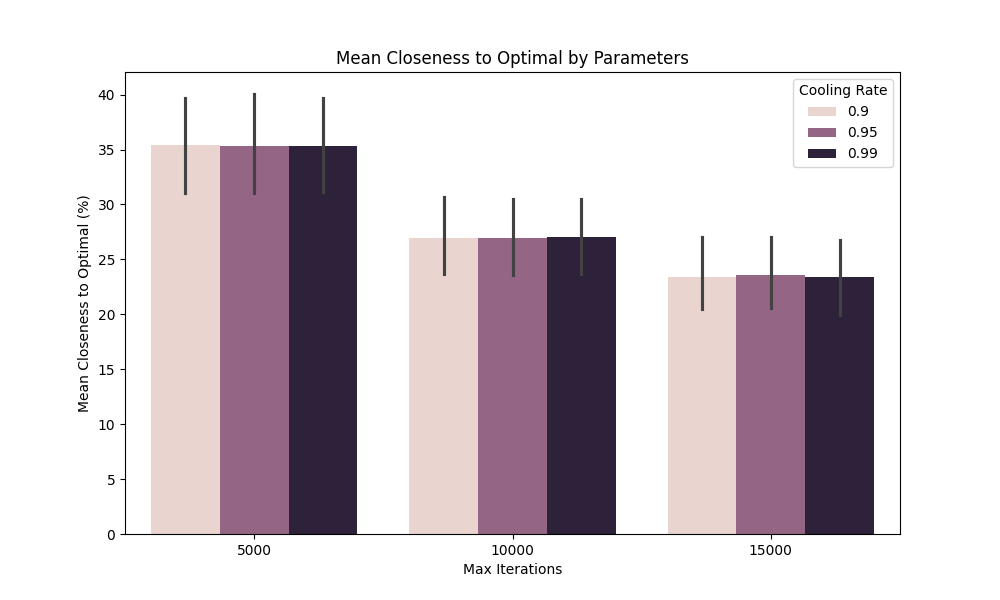
\includegraphics[width=0.8\textwidth]{simulated_annealing/mean_closeness_to_optimal.png}
        \caption{Mean Closeness to Optimal by Parameters}
        \label{fig:mean_closeness}
    \end{figure}

    \subsection{Median Closeness to Optimal}\label{subsec:median-closeness-to-optimal}

    The figure below shows the median closeness to the optimal solution for different parameter settings.

    \begin{figure}[H]
        \centering
        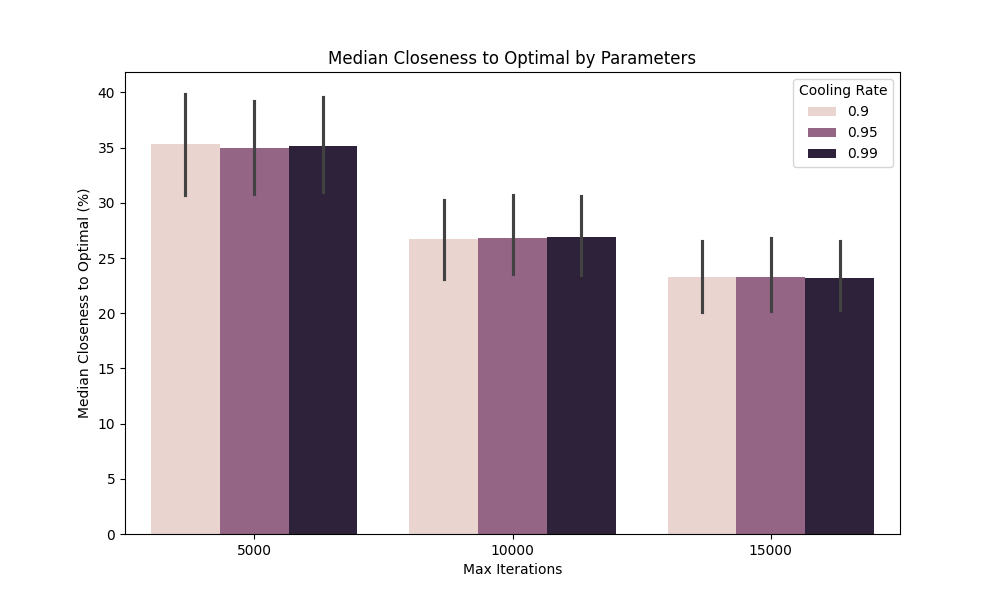
\includegraphics[width=0.8\textwidth]{simulated_annealing/median_closeness_to_optimal.png}
        \caption{Median Closeness to Optimal by Parameters}
        \label{fig:median_closeness}
    \end{figure}

    \subsection{Mean Difference from Optimal}\label{subsec:mean-difference-from-optimal}

    The figure below shows the mean difference from the optimal solution for different parameter settings.

    \begin{figure}[H]
        \centering
        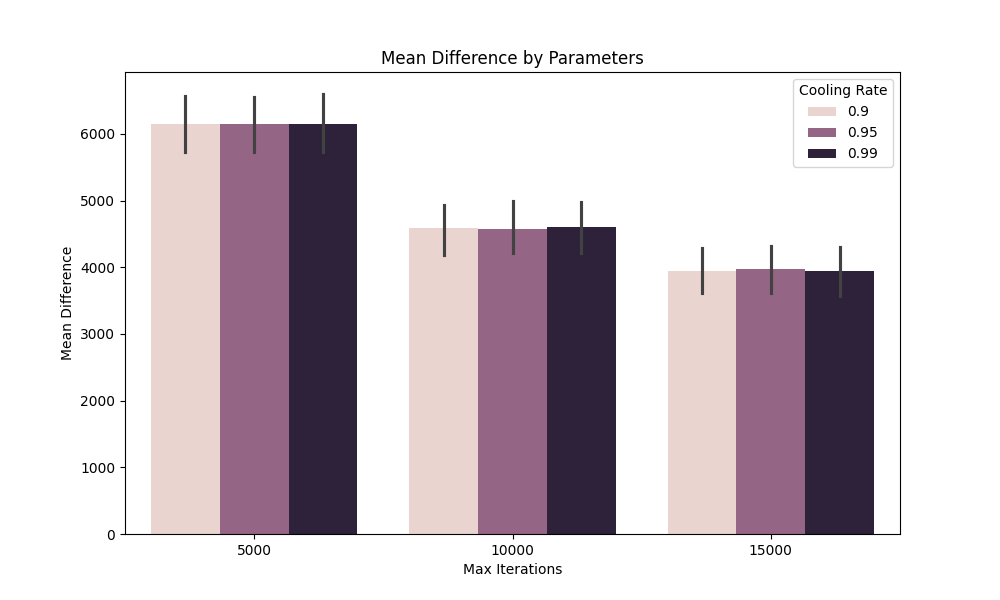
\includegraphics[width=0.8\textwidth]{simulated_annealing/mean_difference.png}
        \caption{Mean Difference from Optimal by Parameters}
        \label{fig:mean_difference}
    \end{figure}

    \subsection{Median Difference from Optimal}\label{subsec:median-difference-from-optimal}

    The figure below shows the median difference from the optimal solution for different parameter settings.

    \begin{figure}[H]
        \centering
        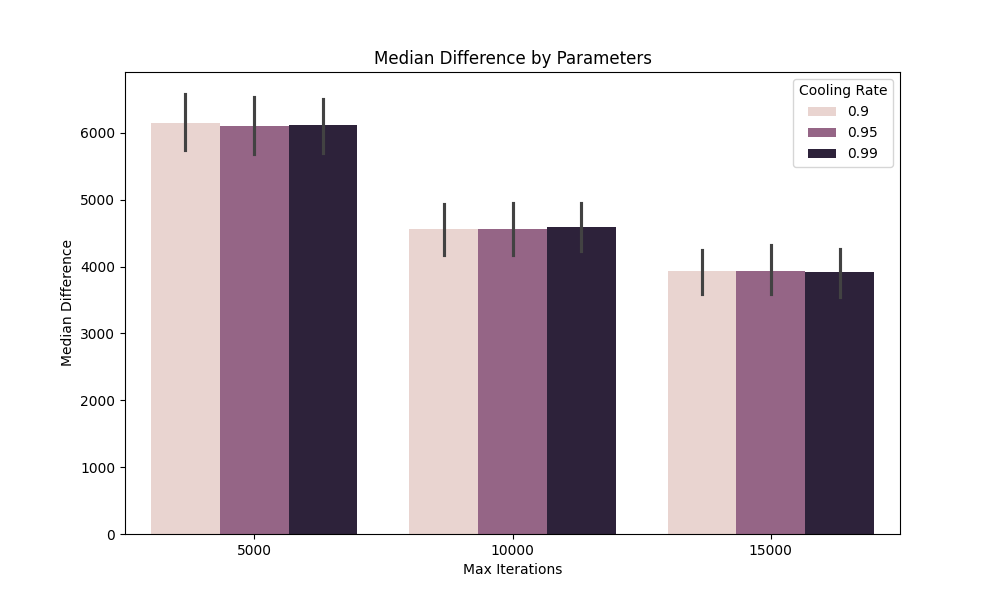
\includegraphics[width=0.8\textwidth]{simulated_annealing/median_difference.png}
        \caption{Median Difference from Optimal by Parameters}
        \label{fig:median_difference}
    \end{figure}

    \subsection{Mean Execution Time}\label{subsec:mean-execution-time}

    The figure below shows the mean execution time for different parameter settings.

    \begin{figure}[H]
        \centering
        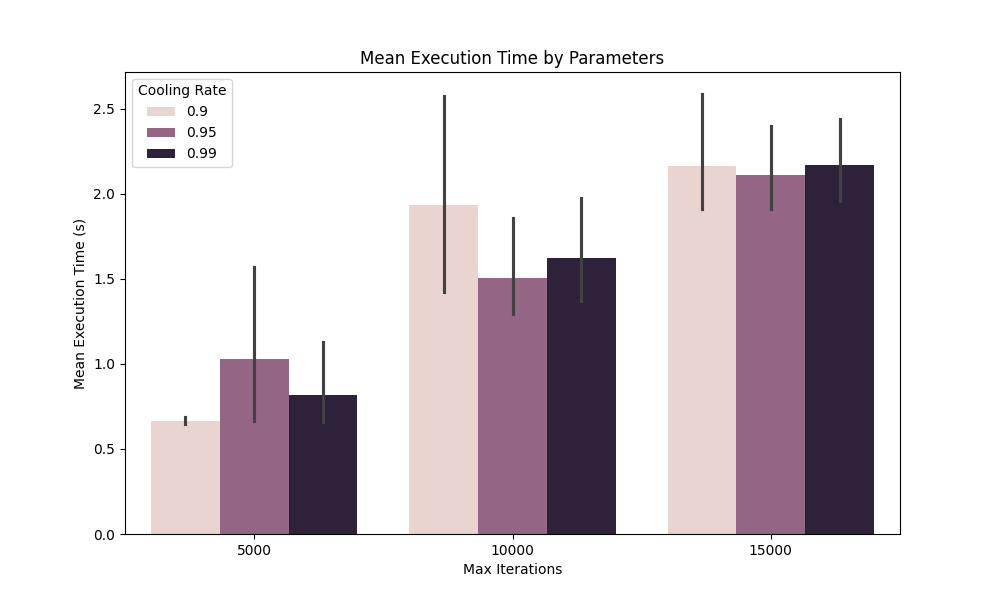
\includegraphics[width=0.8\textwidth]{simulated_annealing/mean_execution_time.png}
        \caption{Mean Execution Time by Parameters}
        \label{fig:mean_execution_time}
    \end{figure}

    \subsection{Median Execution Time}\label{subsec:median-execution-time}

    The figure below shows the median execution time for different parameter settings.

    \begin{figure}[H]
        \centering
        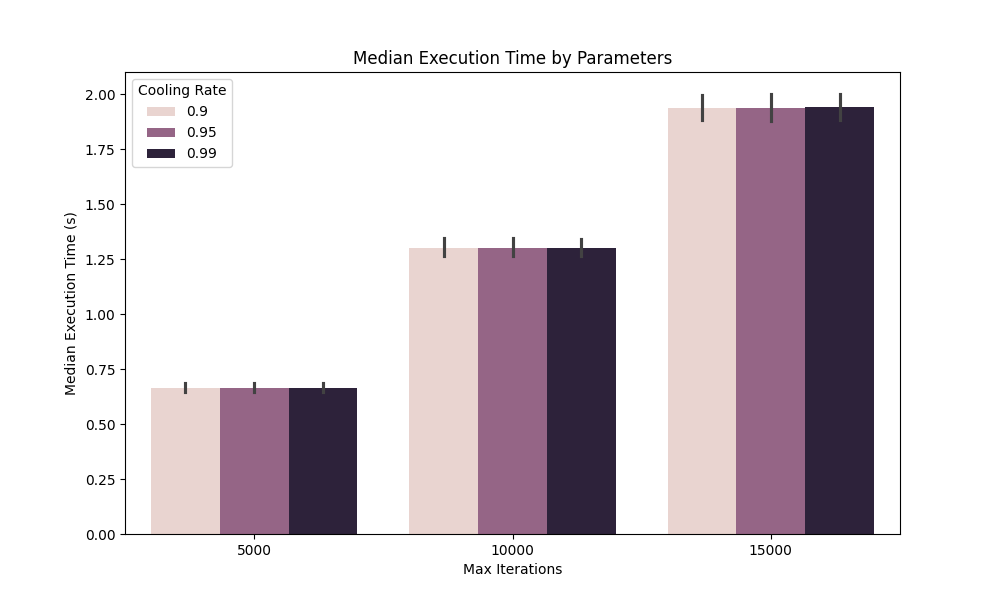
\includegraphics[width=0.8\textwidth]{simulated_annealing/median_execution_time.png}
        \caption{Median Execution Time by Parameters}
        \label{fig:median_execution_time}
    \end{figure}


    \newpage


    \section{Genetic Algorithm Testing and Parameter Optimization}\label{sec:genetic-algorithm-testing-and-parameter-optimization}

    In this section, we present the results of testing various parameter configurations for the Genetic Algorithm (GA) used to solve the Capacitated Vehicle Routing Problem (CVRP). Each dataset was run 20 times with different combinations of population size and generations to ensure robust results. The following metrics were analyzed: mean and median closeness to the optimal solution, mean and median execution time, and mean and median difference from the optimal cost.

    \subsection{Mean Closeness to Optimal by Parameters}\label{subsec:mean-closeness-to-optimal-by-parameters}
    \begin{figure}[H]
        \centering
        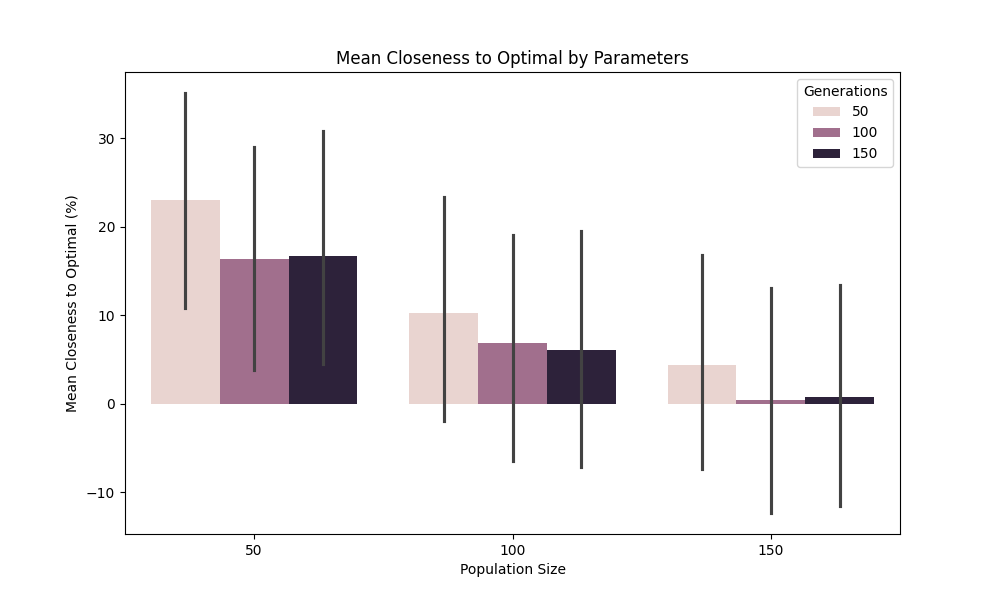
\includegraphics[width=0.8\textwidth]{genetic_algorithm/mean_closeness_to_optimal.png}
        \caption{Mean Closeness to Optimal by Parameters}
        \label{fig:mean_closeness_to_optimal_ga}
    \end{figure}

    The mean closeness to optimal percentage indicates how close, on average, the GA solutions were to the optimal cost across different parameter settings. A lower percentage suggests better performance, with the algorithm generating solutions closer to the optimal. It is observed that configurations with a higher population size and more generations tend to yield results closer to the optimal solution.

    \subsection{Mean Execution Time by Parameters}\label{subsec:mean-execution-time-by-parameters}
    \begin{figure}[H]
        \centering
        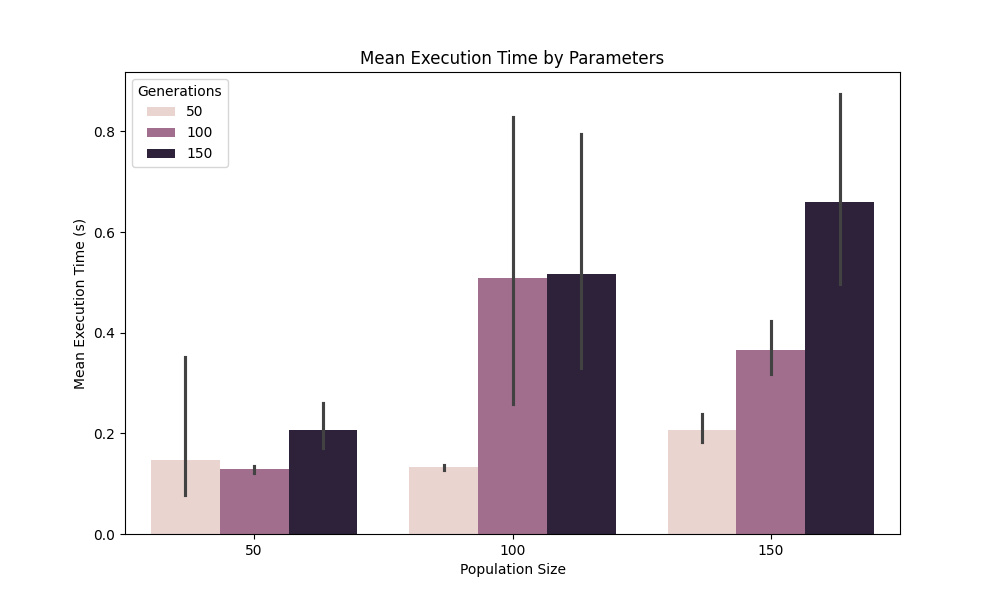
\includegraphics[width=0.8\textwidth]{genetic_algorithm/mean_execution_time.png}
        \caption{Mean Execution Time by Parameters}
        \label{fig:mean_execution_time_ga}
    \end{figure}

    The mean execution time reflects the average computational time taken by the GA to reach a solution. As expected, configurations with higher population sizes and more generations require significantly more computational time. This trade-off between execution time and solution quality is critical for practical applications where time efficiency is crucial.

    \subsection{Mean Difference by Parameters}\label{subsec:mean-difference-by-parameters}
    \begin{figure}[H]
        \centering
        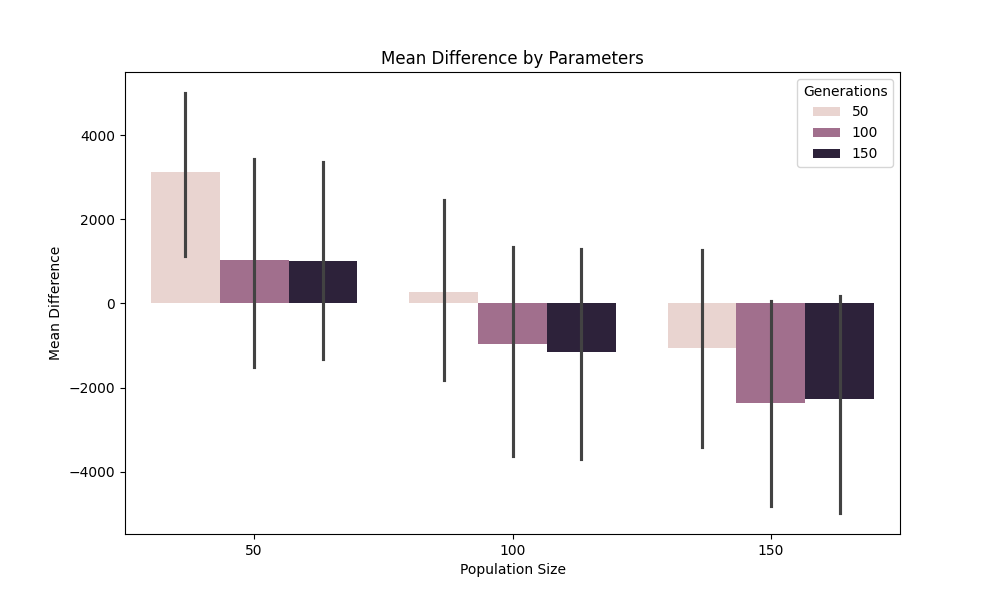
\includegraphics[width=0.8\textwidth]{genetic_algorithm/mean_difference.png}
        \caption{Mean Difference by Parameters}
        \label{fig:mean_difference_ga}
    \end{figure}

    The mean difference metric measures the average deviation of the GA's solutions from the optimal cost. A smaller difference indicates better performance. It is observed that configurations with a larger population size and more generations tend to have a smaller mean difference, indicating better convergence towards the optimal solution.

    \subsection{Median Closeness to Optimal by Parameters}\label{subsec:median-closeness-to-optimal-by-parameters}
    \begin{figure}[H]
        \centering
        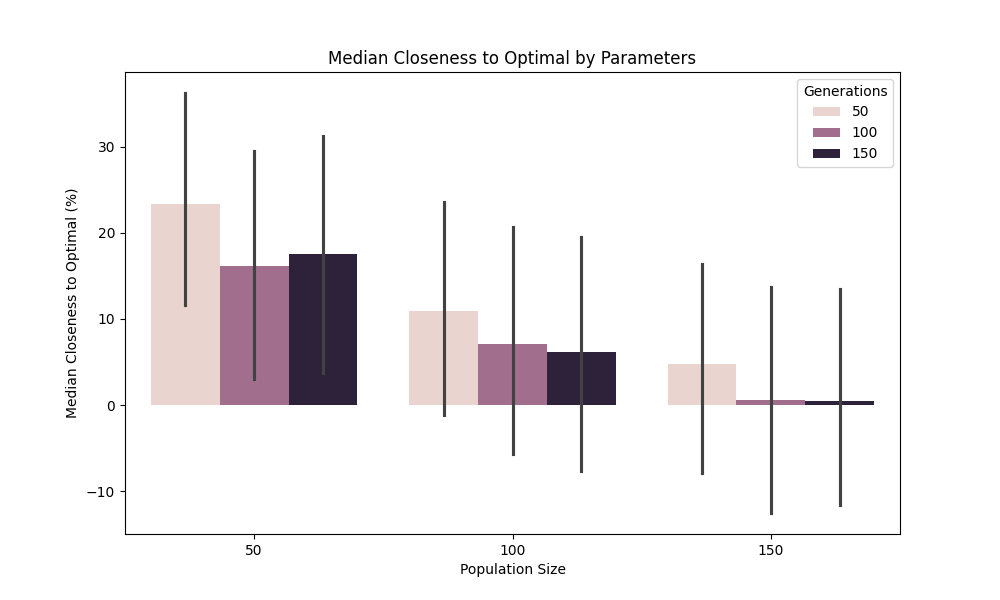
\includegraphics[width=0.8\textwidth]{genetic_algorithm/median_closeness_to_optimal.png}
        \caption{Median Closeness to Optimal by Parameters}
        \label{fig:median_closeness_to_optimal_ga}
    \end{figure}

    The median closeness to optimal percentage provides an additional perspective on the typical performance of the GA. Similar to the mean closeness, lower values indicate better performance. This metric is less affected by outliers, offering a robust measure of the algorithm's typical performance.

    \subsection{Median Execution Time by Parameters}\label{subsec:median-execution-time-by-parameters}
    \begin{figure}[H]
        \centering
        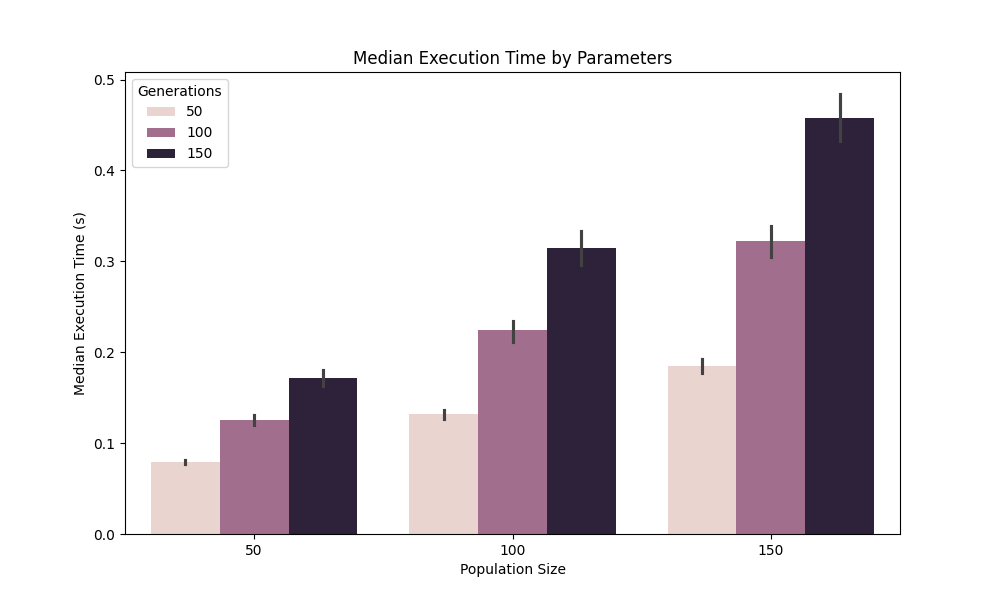
\includegraphics[width=0.8\textwidth]{genetic_algorithm/median_execution_time.png}
        \caption{Median Execution Time by Parameters}
        \label{fig:median_execution_time_ga}
    \end{figure}

    The median execution time offers a robust measure of the typical computational time required by the GA. This metric is particularly useful in understanding the typical time performance, unaffected by extreme values or outliers.

    \subsection{Median Difference by Parameters}\label{subsec:median-difference-by-parameters}
    \begin{figure}[H]
        \centering
        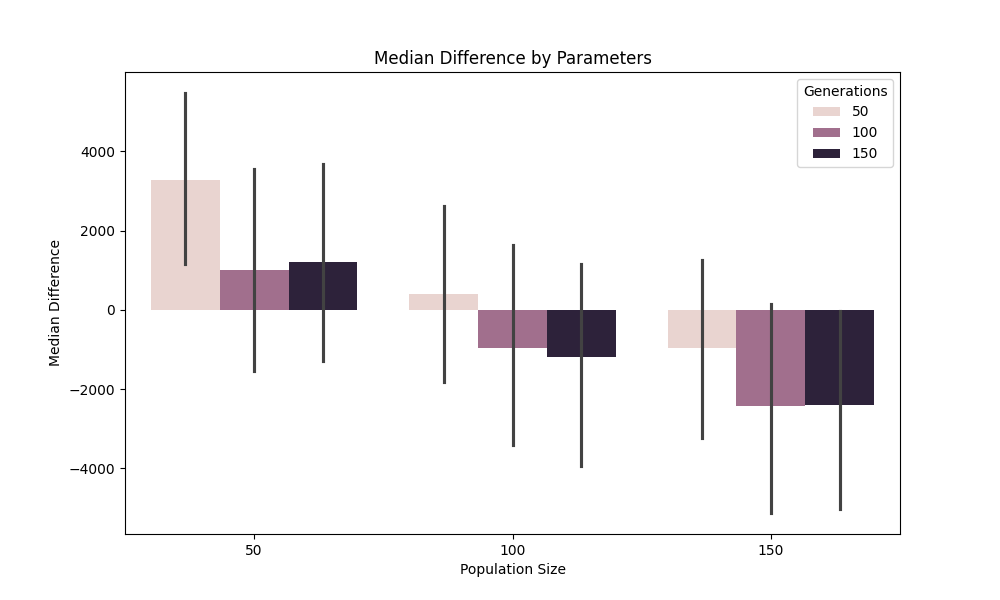
\includegraphics[width=0.8\textwidth]{genetic_algorithm/median_difference.png}
        \caption{Median Difference by Parameters}
        \label{fig:median_difference_ga}
    \end{figure}

    The median difference metric, similar to the mean difference, provides a robust measure of how close the GA solutions typically are to the optimal cost. It is evident that higher population sizes and more generations generally result in a smaller median difference, indicating better solution quality.

    \subsection{F-test Analysis}\label{subsec:f-test-analysis}
    F-tests were conducted to determine if there are significant differences in the means of the different parameter configurations. The results are as follows:
    \begin{itemize}
        \item \textbf{F-test for Closeness to Optimal:} F-statistic = 141.7727433623794, p-value = 3.930721807167456e-232
        \item \textbf{F-test for Execution Time:} F-statistic = 11.038216145823476, p-value = 1.1275732833088738e-15
    \end{itemize}

    The p-values obtained from the F-tests are significantly low, indicating that the differences in means for the different parameter configurations are statistically significant.


    \section{Practical Analysis of Ant Colony Optimization Algorithm}\label{sec:practical-analysis-of-ant-colony-optimization-algorithm}

    In this section, we analyze the performance of the Ant Colony Optimization (ACO) algorithm using various parameters. The algorithm was tested with different combinations of the number of ants and iterations. The key metrics evaluated include the closeness to optimal solution, execution time, and the difference between the total cost and the optimal cost. The following subsections present detailed analysis and visualizations of the results.

    \subsection{Experimental Setup}\label{subsec:experimental-setup}
    The ACO algorithm was tested on several instances, and the parameters used for the tests are as follows:
    \begin{itemize}
        \item Number of ants: 5, 10, 15
        \item Iterations: 10, 20, 30
        \item Decay rate: 0.01
    \end{itemize}
    Each combination of parameters was run multiple times, and the results were aggregated for analysis.

    \subsection{Statistical Analysis}\label{subsec:statistical-analysis}
    The F-test was used to determine the statistical significance of the differences observed in the results based on the different parameter settings. The following F-test results were obtained:
    \begin{itemize}
        \item F-test for Closeness to Optimal: F-statistic = 22.774, p-value = 4.9657e-107
        \item F-test for Execution Time: F-statistic = 10.903, p-value = 7.7767e-45
    \end{itemize}
    The results indicate significant differences in the performance metrics across different parameter settings, as evidenced by the very low p-values.

    \subsection{Visualization of Results}\label{subsec:visualization-of-results}
    The performance metrics were visualized to better understand the impact of the parameters on the ACO algorithm's performance.

    \begin{figure}[H]
        \centering
        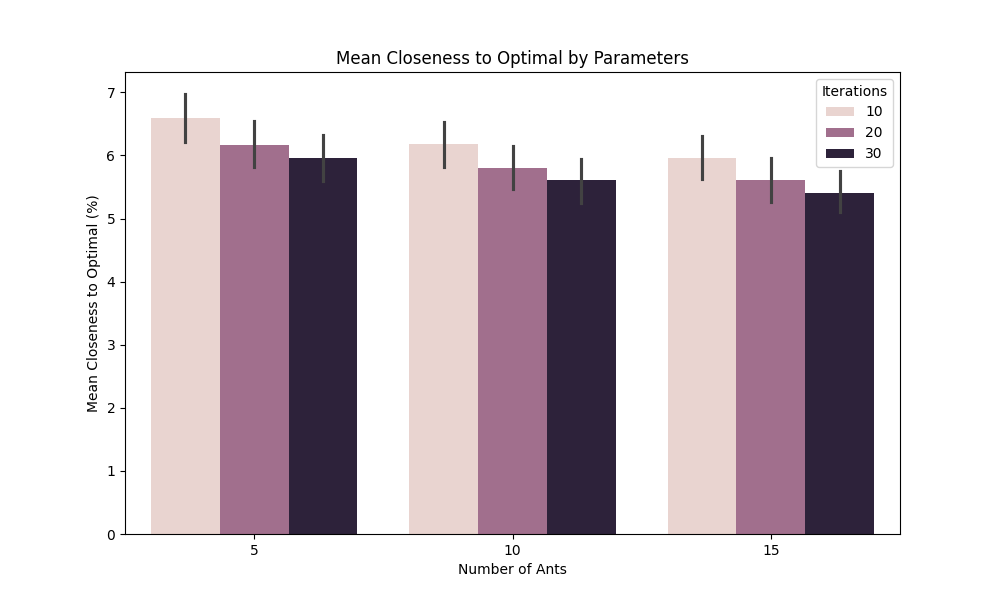
\includegraphics[width=0.8\textwidth]{./aco/aco_mean_closeness_to_optimal.png}
        \caption{Mean Closeness to Optimal by Parameters}
        \label{fig:aco_mean_closeness_to_optimal}
    \end{figure}

    Figure \ref{fig:aco_mean_closeness_to_optimal} shows the mean closeness to the optimal solution across different parameter settings. It can be observed that increasing the number of iterations generally improves the closeness to the optimal solution. However, the number of ants does not significantly affect this metric.

    \begin{figure}[H]
        \centering
        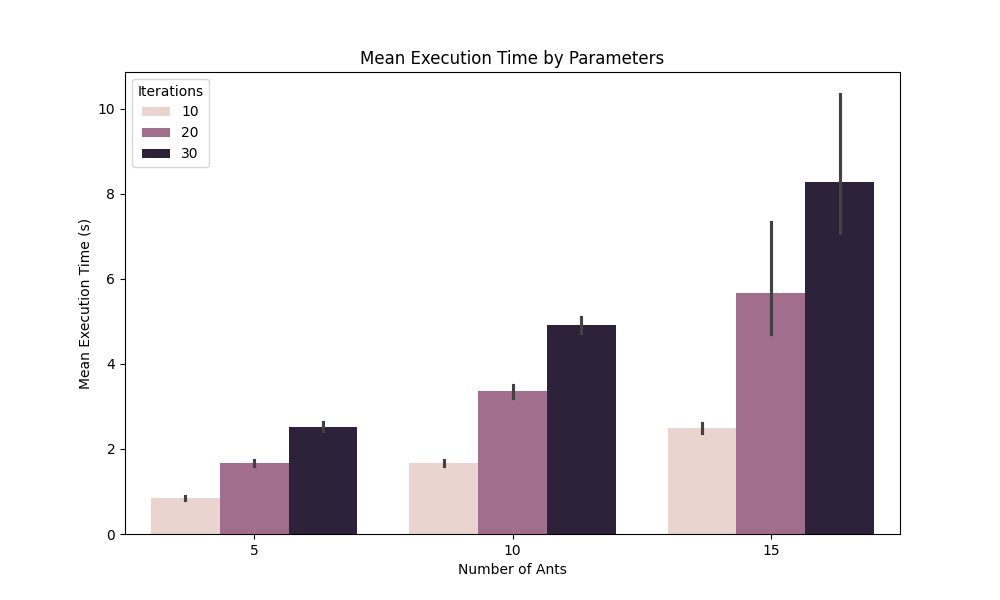
\includegraphics[width=0.8\textwidth]{./aco/aco_mean_execution_time.png}
        \caption{Mean Execution Time by Parameters}
        \label{fig:aco_mean_execution_time}
    \end{figure}

    Figure \ref{fig:aco_mean_execution_time} depicts the mean execution time for the ACO algorithm. As expected, increasing the number of ants and iterations leads to higher execution times. The impact of the number of ants on execution time is more pronounced than the impact of iterations.

    \begin{figure}[H]
        \centering
        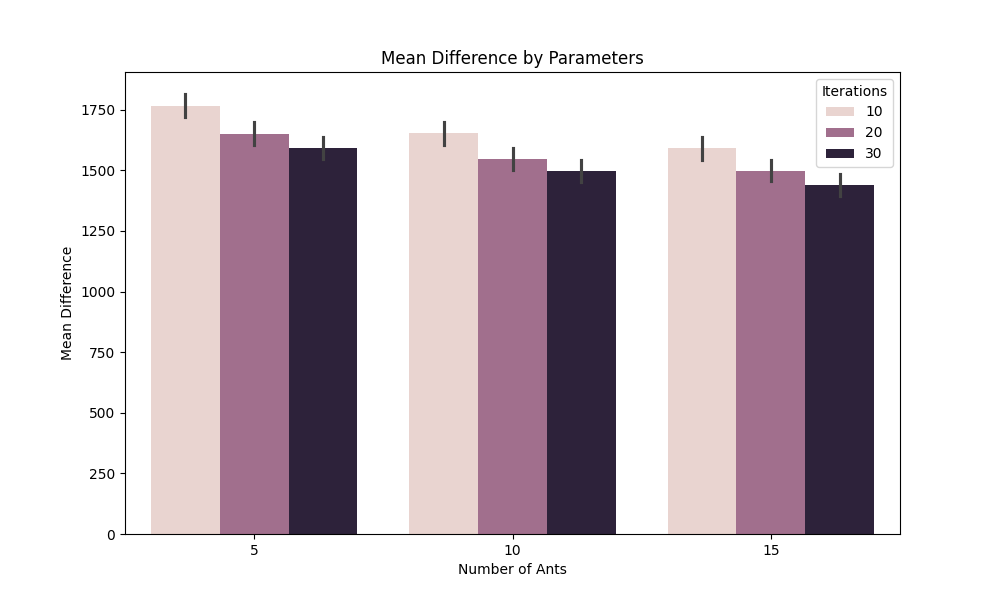
\includegraphics[width=0.8\textwidth]{./aco/aco_mean_difference.png}
        \caption{Mean Difference by Parameters}
        \label{fig:aco_mean_difference}
    \end{figure}

    In Figure \ref{fig:aco_mean_difference}, the mean difference between the total cost and the optimal cost is presented. Similar to the closeness to optimal metric, increasing the number of iterations generally reduces the mean difference, indicating better performance. The number of ants has a lesser impact on this metric.

    \begin{figure}[H]
        \centering
        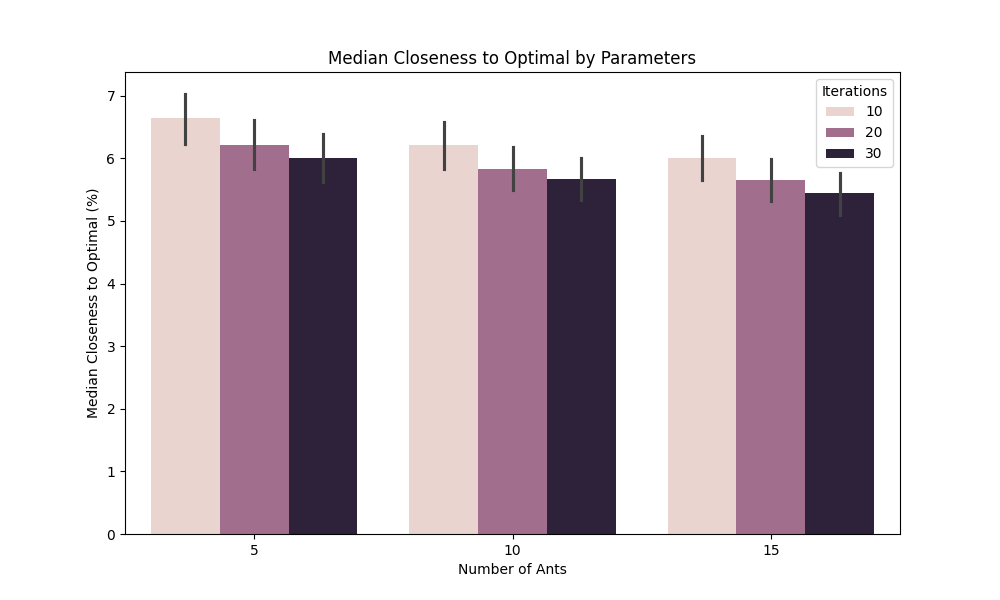
\includegraphics[width=0.8\textwidth]{./aco/aco_median_closeness_to_optimal.png}
        \caption{Median Closeness to Optimal by Parameters}
        \label{fig:aco_median_closeness_to_optimal}
    \end{figure}

    Figure \ref{fig:aco_median_closeness_to_optimal} illustrates the median closeness to the optimal solution. The trends observed are similar to those seen in the mean closeness to optimal, reinforcing the previous observations.

    \begin{figure}[H]
        \centering
        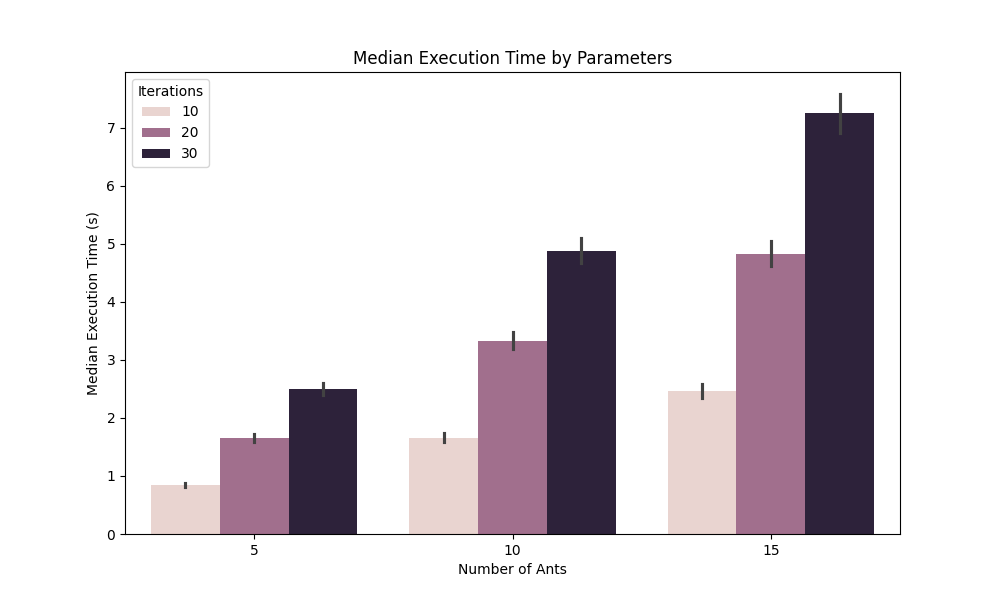
\includegraphics[width=0.8\textwidth]{./aco/aco_median_execution_time.png}
        \caption{Median Execution Time by Parameters}
        \label{fig:aco_median_execution_time}
    \end{figure}

    Figure \ref{fig:aco_median_execution_time} shows the median execution time, which follows similar trends to the mean execution time. This consistency indicates robustness in the execution time metrics across different runs.

    \begin{figure}[H]
        \centering
        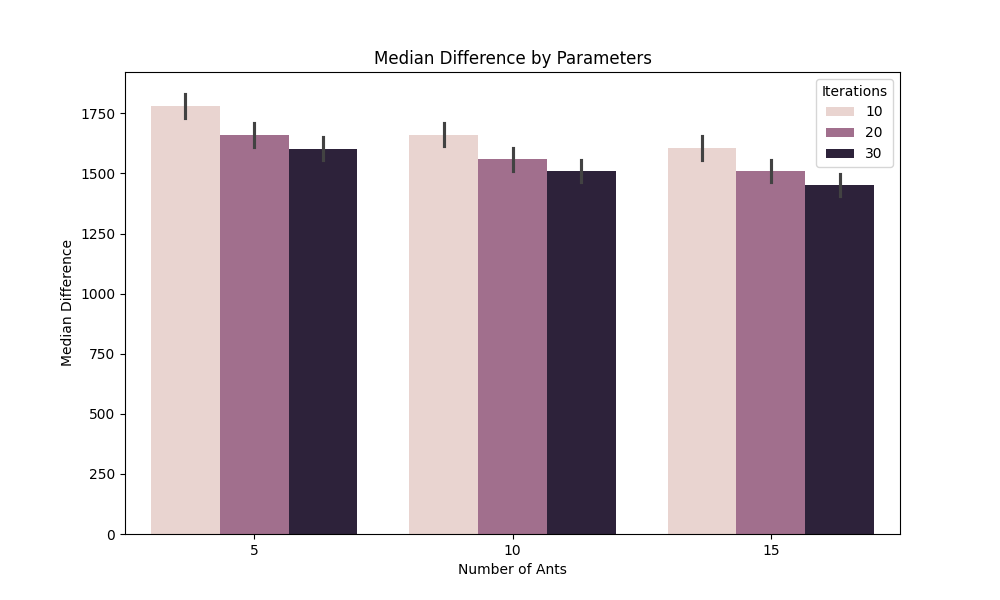
\includegraphics[width=0.8\textwidth]{./aco/aco_median_difference.png}
        \caption{Median Difference by Parameters}
        \label{fig:aco_median_difference}
    \end{figure}

    Lastly, Figure \ref{fig:aco_median_difference} presents the median difference between the total cost and the optimal cost. The median difference also decreases with increasing iterations, suggesting improved performance with more iterations.

    \subsection{Conclusion}\label{subsec:conclusion}
    The analysis demonstrates that the number of iterations significantly affects the performance of the ACO algorithm, with more iterations leading to better closeness to the optimal solution and lower differences from the optimal cost. The number of ants has a lesser, but still noticeable, impact on the execution time. These insights can guide the tuning of ACO parameters for improved performance in solving optimization problems.


%\begin{quote}
%    \emph{Autor/autorka uvedou vlastní název kapitoly vztahující se ke
%    konkrétnímu tématu práce}
%\end{quote}

    \hypertarget{nadpis-uxfarovnux11b-2-2}{%

        \subsection{Nadpis úrovně 2}\label{nadpis-uxfarovnux11b-2-2}}

%\begin{quote}
%    \emph{Obrázek se v textu značí následujícím způsobem: samotný obrázek se
%    označí: „\textbf{Obrázek 1: Název obrázku}`` (11 nebo 12 pt, černě,
%        tučně). Obrázky se označují názvem a číslováním nad obrázkem a zdrojovým
%        dokumentem pod obrázkem, příp. informace o vlastním zpracování (11 nebo
%        12 pt, černě). K popisování doporučujeme využít nástroje textového
%        editoru, který usnadní generování seznamu obrázků na konci práce.}
%\end{quote}



    \newpage
    \hypertarget{zuxe1vux11br}{%


        \section{Závěr}\label{zuxe1vux11br}}

    \begin{quote}
        Rozsah je zpravidla 5-10 normostran.
    \end{quote}

    \newpage
    \hypertarget{seznam-pouux17eituxfdch-zdrojux16f}{%
        \section{Seznam použitých
        zdrojů}\label{seznam-pouux17eituxfdch-zdrojux16f}}

    \begin{quote}
        V~seznamu zdrojů musí být uvedeny všechny v~závěrečné práci citované
        zdroje. Zároveň nesmí seznam obsahovat zdroje, které nejsou v~závěrečné
        práci použity.

        Používáme citační normu ČNS ISO 690. Doporučujeme pro tvorbu citací
        některý z~citačních nástrojů, které jsou v~základní verzi zpravidla
        zdarma dostupné.
    \end{quote}

    \newpage
    \hypertarget{seznam-obruxe1zkux16f-existujuxed-li}{%
        \section{Seznam obrázků
            (existují-li)}\label{seznam-obruxe1zkux16f-existujuxed-li}}

    \begin{quote}
        Obrázek 1: Logo 11

        Obrázek 2: Obrázek jednorožce 12

        \newpage
        \textbf{Seznam tabulek (existují-li)}

        \protect\hyperlink{_bookmark9}{Tabulka 1: Statistika vět zachovaných a
        vyřazených filtr. kritériem \emph{FK1} 12}
    \end{quote}

    \newpage
    \hypertarget{seznam-grafux16f-existujuxed-li}{%
        \section{Seznam grafů
            (existují-li)}\label{seznam-grafux16f-existujuxed-li}}

    \newpage
    \hypertarget{seznam-pux159uxedloh-existujuxed-li}{%
        \section{Seznam příloh
            (existují-li)}\label{seznam-pux159uxedloh-existujuxed-li}}

    \begin{quote}
        \emph{Každá příloha musí být alespoň jednou odkázána do vlastního textu
        práce. Přílohy se číslují. Každá příloha začíná na nové stránce.}
    \end{quote}

    \newpage
    \hypertarget{pux159uxedloha-a-nuxe1zev-pux159uxedlohy}{%
        \section{Příloha A -- Název
        přílohy}\label{pux159uxedloha-a-nuxe1zev-pux159uxedlohy}}

    \newpage
    \hypertarget{pux159uxedloha-b-nuxe1zev-pux159uxedlohy}{%
        \section{Příloha B -- Název
        přílohy}\label{pux159uxedloha-b-nuxe1zev-pux159uxedlohy}}

\end{document}
